% Chapter 3

\chapter{Geles polim\'ericos} % Main chapter title

\label{Chapter3} % For referencing the chapter elsewhere, use \ref{Chapter1} 

%----------------------------------------------------------------------------------------

% Define some commands to keep the formatting separated from the content 
\newcommand{\keyword}[1]{\textbf{#1}}
\newcommand{\tabhead}[1]{\textbf{#1}}
\newcommand{\code}[1]{\texttt{#1}}
\newcommand{\file}[1]{\texttt{\bfseries#1}}
\newcommand{\option}[1]{\texttt{\itshape#1}}

%----------------------------------------------------------------------------------------




\section{Modelo de 2 fases}

Los microgeles son part\'iculas blandas hechas de cadenas de pol\'imeros entrecruzados que pueden mostrar un comportamiento tanto coloidal como macromolecular \cite{plamper2017functional}.
Inmersas en soluciones acuosas, estas part\'iculas incorporan y retienen grandes cantidades de agua dentro de su estructura polim\'erica.
Por lo general, sus di\'ametros van desde decenas de nan\'ometros (nanogeles) hasta varias micras.
Sin embargo, la caracter\'istica m\'as llamativa de estas part\'iculas es su capacidad para absorber o liberar solventes y cambiar de tama\~no en respuesta a una variedad de est\'imulos externos.
Este comportamiento de respuesta es  generlmente reversible y depende de la composici\'on qu\'imica de la red polim\'erica.


Por ejemplo los microgeles compuestos por cadenas polim\'ericas que tienen segmentos \'acidos como el \'acido acr\'ilico o metacr\'ilico (AA y MAA, respectivamente) se hinchan/deshinchan muchas veces en respuesta a cambios en el pH de la soluci\'on que los contienen \cite{snowden1996colloidal}.
El pH en el cual se marca el inicio y caracteriza esta transici\'on es el pKa aparente del microgel, que depende de la concentraci\'on de sal de la soluci\'on y frecuentemente difiere del pKa intrínseco del mon\'omero \'acido.
Estos microgeles tambi\'en ajustan su tama\~no en respuesta a cambios en la concentraci\'on de sal de la soluci\'on \cite{snowden1996colloidal}.

An\'alogamente, los microgeles de algunos pol\'imeros termosensibles experimentan una transici\'on de fase de volumen (VPT por sus siglas en ingl\'es) cuando se calientan por encima de una temperatura caracter\'istica (VPTT o $T_{pt}$) \cite{Pelton1986,Pelton2000}.
Este comportamiento se origina porque tales pol\'imeros son insolubles en agua por encima de cierta temperatura de soluci\'on cr\'itica m\'as baja (LCST) \cite{Kawaguchi2020}.
Normalmente, la LCST del pol\'imero y la VPTT de la red  son aproximadamente id\'enticas. 
Este es el caso de las part\'iculas de microgel de poli(N-isopropilacrilamida) (PNIPAm) \cite{Pelton1986}, cuyo volumen colapsa por encima de $32 C$, siendo le mismo para el  pol\'imero lineal \cite{Schild1992}.

Al tener un VPTT alrededor de la temperatura corporal, los microgeles de PNIPAm han generado un gran inter\'es para aplicaciones biom\'edicas \cite{Guan2011}.
Las estrategias para controlar el VPTT de los microgeles incluyen la s\'intesis de nuevos mon\'omeros termosensibles  \cite{Cai2007,Macchione2019}, as\'i como la copolimerizaci\'on con un mon\'omero i\'onico o ionizable  \cite{Hirose1987,Lopez2020}.
Este \'ultimo enfoque produce microgeles de respuesta m\'ultiple que son susceptibles a cambios en la temperatura, el pH y la concentraci\'on de sal  \cite{snowden1996colloidal, Farooqi2017}.
Los microgeles de NIPAm y AA han sido ampliamente estudiados \cite{Morris1997, Jones2000,Bradley2005,Begum2016};
Tambi\'en se han investigado microgeles de copol\'imeros de NIPAm y MAA  \cite{Dowding2000,Hoare2004,Giussi2015}.
El VPTT de estos microgeles de respuesta m\'ultiple depende del pH de la soluci\'on y la concentraci\'on de sal, y la fracci\'on de mon\'omero ionizable en las cadenas de pol\'imero  \cite{Morris1997,Jones2000, Hoare2004, Bradley2005, Lee2008,Wong2009,Hamzavi2016}.
Adem\'as, la incorporaci\'on del comon\'omero \'acido proporciona un mecanismo controlado por el pH para la captaci\'on/liberaci\'on de mol\'eculas con carga opuesta, lo que hace que los microgeles de respuesta m\'ultiple sean atractivos para el dise\~no de sistemas funcionales de administraci\'on de f\'armacos \cite{Liu2017}.

Las aplicaciones basadas en microgeles polim\'ericos son cada vez m\'as diversas y cada vez m\'as importantes en diferentes \'areas de la tecnolog\'ia \cite{plamper2017functional}.
Los nanocompuestos hechos de microgeles de poli(NIPAm-\emph{co}-MAA) que incorporan nanopart\'iculas de oro o plata o redes metal organicas (MOF)tienen aplicaciones potenciales en el desarrollo de materiales con actividad catal\'itica  para la degradación de contaminantes industriales  \cite{Khan2013synthesis,Shi2014,Allegretto2020}.
Estos microgeles tambi\'en se pueden aplicar para el desarrollo de emulsiones sensibles al pH, la sal y la temperatura \cite{Ngai2005,Ngai2006, Brugger2008, Schmidt2011} o como plantillas para el ensamblaje de nanomateriales \cite{Wong2009}.
Los geles polim\'ericos de tama\~no nano/micro de respuesta m\'ultiple son excelentes candidatos para el desarrollo de aplicaciones biom\'edicas m\'inimamente invasivas, incluida la ingeniería de tejidos  \cite{Daly2020}
 \citet{Culver2017A}han utilizado nanogeles de poli(NIPAm-co-MAA) funcionalizados para la uni\'on y detecci\'on de diferentes prote\'inas.
Recientemente se investigaron dispositivos basados en microgeles de poli(NIPAm-co-MAA) para la encapsulación/liberaci\'on del f\'armaco quimioterap\'eutico Doxorrubicina \cite{Giussi2020, MartinezMoro2020, Pergushov2020}.

En este contexto, en este cap\'itulo mostramos el desarrollo de una teor\'ia de equilibrio de dos fases y realizamos una investigaci\'on sistem\'atica del comportamiento termodin\'amico de microgeles compuestos de copol\'imeros aleatorios de NIPAm y un comon\'omero \'acido (MAA).
Este modelo describe la qu\'imica f\'isica detr\'as de todos los fen\'omenos de hinchamiento del microgel impulsado por el pH, la dependencia no monot\'onica del tama\~no de part\'icula de la concentraci\'on de sal y el colapso de la red al aumentar la temperatura por encima del VPTT.
Las predicciones que mosntramos brindan una imagen clara de los efectos de la composici\'on de la soluci\'on (pH, concentración de sal) y la qu\'imica del pol\'imero (contenido de MAA, grado de entrecruzamiento) en el VPT.
Tambi\'en investigamos las mejores condiciones para la encapsulaci\'on de doxorrubicina y daunorrubicina dentro de estos microgeles.
Los c\'alculos  ac\'a mostrados son espec\'ificos para el \'acido metacr\'ilico con $pKa = 4,65$, pero el comportamiento fisicoqu\'imico informado puede describir cualitativamente una variedad de microgeles basados en NIPAm que se han modificado con otros mon\'omeros \'acidos que tienen diferente pka y diferente solubilidad a pH bajo.


El comportamiento de los microgeles de poli(NIPAm-co-MAA), incluido su VPT y la interacci\'on con pol\'imeros de carga opuesta, se ha descrito utilizando una variedad de t\'ecnicas experimentales \cite{Hoare2004,Dowding2000,Kleinen2008,Kleinen2010, Giussi2015, Su2016,Giussi2020}.
Tambi\'en se han aplicado teor\'ias  y simulaciones moleculares de grano grueso para investigar el comportamiento de los microgeles polim\'ericos sensibles a est\'imulos \cite{quesada2011gel,ahualli2016coarse,Landsgesell2019SM}.
Estos trabajos se han centrado principalmente en el hinchamiento y otras propiedades de las part\'iculas que tienen una red de pol\'imero permanentemente cargada , y algunos han abordado el efecto de la temperatura y la calidad del solvente \cite{Jha2011, QuesadaPerez2013, moncho-jorda2016a, ahualli2016coarse, AdroherBenitez2017PCCP}.
Recientemente, estudios  con simulaciones han considerado la respuesta al pH de microgeles compuestos de pol\'imeros reguladores de carga \cite{Schroeder2015,Rud2017,Sean2018, Hofzumahaus2018,Lu2019}.
Sin embargo, solo unos pocos trabajos te\'oricos han investigado las propiedades de los microgeles de respuesta m\'ultiple en funci\'on de la temperatura, el pH y la concentración de sal  \cite{CaprilesGonzalez2008,polotsky2013collapse}.


\subsection{Fase Microgel}\label{sec:theory}
%%%%%%%%%%%%%%%%%%%%%%%%%%%%%%%%%%%%%%%%%%%%%%%%%%%%%%%%%%%%%%%%%%%%%


Consideremos un modelo de dos fases: un microgel de poli(NIPAm-\emph{co}-MAA) (P(NIPAm-MAA)) (la fase $1$, denotada por $MG$) en contacto con una soluci\'on acuosa ( fase $2$, denotada por $s$).
Externamente, podemos controlar la temperatura $T$, el pH y la concentraci\'on de sal de esta soluci\'on, lo que da como resultado que el microgel tenga un radio $R$ y un volumen $V=\frac{4}{3}\pi R^3$.
El potencial termodin\'amico cuyo m\'inimo produce las condiciones de equilibrio dentro de la fase de microgel es un  potencial semi gran can\'onico, $\Omega_{MG}$.
%
\begin{align}
    \begin{aligned}
       \Omega_{MG}=& -TS_{mez} + F_{qca,MAA} +  F_{ela}\\
       & + U_{elec}+  U_{ste} + U_{VdW} -{\sum_{\gamma}
        {\mu_\gamma N_\gamma}}
    \end{aligned}
    \label{eq:gel:free-energy-implicit}
\end{align}
%

\noindent En donde $S_{mez}$ es la entropí\'ia de traslaci\'on (mezcla) de las especies libres en la fase de microgel: mol\'eculas de agua ($w$), hidronio ($H_3O^+$) e iones de hidr\'oxido ($OH^-$ ), y cationes de sal ($+$) y aniones ($-$).
Hemos considerado una sal monovalente, $KCl$,  completamente disociada en iones de potasio y cloruro.

\begin{align}
-\frac{S_{mez}}{k_B}	= \sum_{\gamma} \rho_\gamma\left(\ln\left(\rho_\gamma v_w\right) -1 + \beta\mu^0_\gamma\right) 
\end{align}

\noindent en donde  $\beta=\frac{1}{k_BT}$ , $T$ es la temperatura del sisteman y  $k_B$ es la constante de Boltzmann.
La densidad num\'erica de la especie $\gamma$ es $\rho_\gamma$ y $\mu^0_\gamma$ es su potencial qu\'imico est\'andar,  $v_w$ es el volumen de una mol\'ecula de agua.

$F_{qca,MAA}$ es la energ\'ia química libre que describe la protonaci\'on de equilibrio de las unidades de MAA.


\begin{align}
	\beta F_{qca, MAA} =  \frac{\phi_{MAA}}{v_{MAA}} \left[f(\ln f+ \beta\mu^0_{MAA^-}) +(1-f)(\ln (1-f)+\beta\mu^0_{MAAH})\right]
\end{align}


\noindent donde $\phi_{MAA}$ es la fracci\'on de volumen que ocupan estos segmentos, $v_{MAA}$ es el volumen de este segmento, y $f$ es el grado de disociaci\'on del mismo. 
La fracci\'on de volumen de los segmentos MAA cargados es $f\phi_{MAA}$, y la de las unidades protonadas (o sin carga) es $(1-f)\phi_{MAA}$.
Los potenciales qu\'imicos est\'andar son $\mu^0_{MAA^-}$ y $\mu^0_{MAAH}$ para las especies desprotonadas(cargadas) y protonadas, respectivamente.
Utilizamos el t\'ermino segmento para identificar las unidades qu\'imicas que componen las cadenas polim\'ericas (MAA y NIPAm).


$F_{ela}$ es la energ\'ia libre el\'astica que explica la libertad conformacional de la red polim\'erica.

\begin{align}
	\beta F_{ela} = \dfrac{3}{2}\dfrac{N_{seg}}{n_{ch} V}\left[\left(\dfrac{R}{R_0}\right)^2 - \ln\dfrac{R}{R_0} -1\right]
\end{align}

Esta expresi\'on se describe en \cite{moncho-jorda2016a} y proviene del modelo de elasticidad del caucho,
donde $N_{seg}$ es el n\'umero total de segmentos en la red de pol\'imero y $n_{ch}$ es el n\'umero de segmentos por cadena de pol\'imero o \emph{longitud de cadena}.
La constante de elasticidad en esta energ\'ia es proporcional al cociente $\dfrac{N_{seg}}{n_{ch}}$, que representa el n\'umero (total) de cadenas de pol\'imero en el microgel.
El radio del microgel seco es $R_0$, lo que satisface con la expresi\'on:

%
%
\begin{align}
	\begin{aligned} 
		\dfrac{4}{3}\pi R_0^3=V_0&=N_{seg}\Big( x_{MAA} v_{MAA}\\
		&\qquad+x_{NIPAm} v_{NIPAm}\Big)
	\end{aligned}
\end{align}


\noindent donde $V_0$ es el volumen de la part\'icula seca; $x_{MAA}$ y $x_{NIPAm}$ son la fracci\'on de los segmentos MAA y NIPAm, respectivamente.
Entonces, el n\'umero total de segmentos MAA es $x_{MAA}N_{seg}$ y el de unidades NIPAm es $x_{NIPAm}N_{seg}$, cada uno con un volumen $v_{NIPAm}$.
Los microgeles que consideramos aqu\'i satisfacen $x_{NIPAm}=1-x_{MAA}$.



$U_{elec}$ y $U_{ste}$ representan respectivamente las interacciones electrost\'aticas y las repulsiones est\'ericas.

\begin{align}
	  \beta U_{elec} =\left(\sum_{\gamma } {\rho_\gamma q_\gamma + f\dfrac{\phi_{MAA}}{v_{MAA}}q_{MAA}}\right)\beta\psi_{MG}
\end{align}

\noindent donde $q_\gamma$ y $q_{MAA}$ son la carga el\'ectrica de las moléculas $\gamma$ y los segmentos MAA, respectivamente.
El potencial electrost\'atico dentro de la fase de microgel es $\psi_{MG}$. Fuera de esta fase el potencial es nulo $\psi_s = 0$

En donde se impone una restriccio\'on de electroneutralidad del microgel, que puede expresarse como:
%
%
\begin{align}
	\begin{aligned}
		\sum_{\gamma  } \rho_\gamma q_\gamma + f\frac{\phi_{MAA}}{v_{MAA}}q_{MAA}=0
	\end{aligned}
	\label{eq:gel:charge-neutrality}
\end{align}

Las interacciones stericas se incorporan como una segunda restricci\'on al sistema, la cual consiste en que  el volumen del microgel est\'a completamente ocupado por los segmentos de la red y las especies quí\'icas libres.

%
\begin{align}
	\begin{aligned}
		\sum_{\gamma } \rho_\gamma v_\gamma  + \phi_{MAA} + \phi_{NIPAm} = 1
	\end{aligned}
	\label{eq:gel:packing}
\end{align}



\noindent donde $v_\gamma$  es el volumen molecular de la especie $\gamma$, y la fracci\'on de volumen de cada componente de la red son: 
%
%
\begin{align}
	\phi_{MAA}&=N_{seg}\dfrac{x_{MAA}v_{MAA}}{\frac{4}{3}\pi R^3}\\
	\phi_{NIPAm}&=N_{seg}\dfrac{x_{NIPAm}v_{NIPAm}}{\frac{4}{3}\pi R^3}
\end{align}



$U_{VdW}$ es la contribuci\'on que describe las interacciones efectivas pol\'imero-disolvente; para este trabajo hemos realizado la siguiente aproximaci\'on: 
\begin{align}
	U_{VdW} = U_{NIPAm-w} + U_{MAA-w}
\end{align}
\noindent en donde $U_{NIPAm-w}$ incorpora la transici\'on hidrofílica-hidrof\'obica de NIPAm al aumentar la temperatura por encima de su temperatura de transici\'on cr\'itica. 
Del mismo modo $U_{MAA-w}$ hace cuenta de la interacci\'on entre los segmentos de MAA y agua.
Los resultados presentes en este cap\'itulo consideran a los segmentos de $MAA$ completamente hidrofilicos y por tanto $U_{MAA-w} = 0$

\begin{align}
	\beta U_{VdW} = U_{NIPAm-w} = \chi (T, \phi_{NIPAm})\rho_w \phi_{NIPAm}
\end{align}


Este  t\'ermino explica la respuesta de PNIPAm a los cambios de temperatura a trav\'es de un par\'ametro de interacci\'on pol\'imero solvente, $\chi$, que depende de la temperatura y la fracci\'on de volumen de NIPAm, $\phi_{NIPAm}$.
Seg\'un  \cite{afroze2000}, este par\'ametro de Flory-Huggins se puede expresar como:
%
%


\begin{align}
	\begin{aligned}
		\chi (T, \phi_{NIPAm}) &=g_0(T) +g_1(T)\phi_{NIPAm} \\
		&~+ g_2(T)\phi_{NIPAm}^2
	\end{aligned}
\end{align}

\noindent con
%
%
\begin{align}
	\begin{aligned} 
		g_k(T)=g_{k0} + \frac{g_{k1}}{T} + g_{k2}T
	\end{aligned}
\end{align}


\noindent para  $k=0,1,2$, los coeficinetes son: $g_{00}= -12.947$, $g_{02}=0.044959\,$K$^{-1}$, $g_{10}= 17.920$, $g_{12}= -0.056944$\,K$^{-1}$, $g_{20}= 14.814$, $g_{22}= -0.051419$\,K$^{-1}$  y $g_{k1}\equiv 0$ \cite{afroze2000}




Finalmente, la suma sobre  $\gamma$ expresa el equilibrio qu\'imico con la fase de soluci\'on, donde $\mu_\gamma$ y $N_\gamma$ son el potencial qu\'imico y el n\'umero de mol\'eculas de la especie $\gamma$, respectivamente.
Aqu\'i, el subíndice $\gamma$ identifica  las especies qu\'imicas libres, $\gamma \in \left\{ w, H_3O^+, OH^-, +,- \right\}$.
Hay que tener en cuenta que $\Omega_{MG}$ es un potencial semi-gran can\'onico porque la fase de microgel puede intercambiar cada una de estas mol\'eculas con la fase de soluci\'on, mientras que la red de pol\'imero está confinada dentro de la primera.


\begin{align}
	\sum_\gamma N_\gamma \mu_\gamma = \sum_{\gamma }{\rho_\gamma\beta\mu_\gamma}
	+ \beta\mu_{H^+}(1-f)\dfrac{\phi_{MAA}}{v_{MAA}}
\end{align}

Esta contribuci\'on muestra el equilibrio qu\'imico entre el microgel y la fase de soluci\'on, donde el segundo t\'ermino representa a los protones asociados a unidades de MAA;
a saber, $\mu_{H^+}\equiv\mu_{H_3O^+}$ se conjuga con el n\'umero total de protones,
$N_{H_3O^+}+N_{MAAH}=V\left(\rho_{H_3O^+}+(1-f)\dfrac{\phi_{MAA}}{v_{MAA}}\right)$.


La forma expl\'icita del potencial termodin\'amico es:




%
\begin{align}
\begin{aligned}
\beta&\frac{\Omega_{MG}(R)}{V}=\\& ~ \sum_{\gamma} \rho_\gamma\left(\ln\left(\rho_\gamma v_w\right) -1 + \beta\mu^0_\gamma\right) \\
& + \frac{\phi_{MAA}}{v_{MAA}} \left[f(\ln f+ \beta\mu^0_{MAA^-})\right.\\
&\qquad\left.+(1-f)(\ln (1-f)+\beta\mu^0_{MAAH})\right] \\
%
& + \dfrac{3}{2}\dfrac{N_{seg}}{n_{ch} V}\left[\left(\dfrac{R}{R_0}\right)^2 - \ln\dfrac{R}{R_0} -1\right] \\
%
& +  \left(\sum_{\gamma } {\rho_\gamma q_\gamma + f\dfrac{\phi_{MAA}}{v_{MAA}}q_{MAA}}\right)\beta\psi_{MG}\\
%
& +\beta\pi_{MG} \left[ \sum_{\gamma } \rho_\gamma v_\gamma  + \phi_{MAA} + \phi_{NIPAm} -1 \right] \\
%
& + \chi (T, \phi_{NIPAm})\rho_w \phi_{NIPAm} \\
%
& -\sum_{\gamma }{\rho_\gamma\beta\mu_\gamma}
 -\beta\mu_{H^+}(1-f)\dfrac{\phi_{MAA}}{v_{MAA}}\\
%
%
\end{aligned}
\label{eq:gel:free-energy}
\end{align}




\noindent En donde $\pi_{MG}$ es la presi\'on osm\'otica de la fase de microgel, introducido como un multiplicador de Lagrange para imponer la restricci\'on de incompresibilidad, ec. \ref{eq:gel:packing}.


Nuestro potencial termodin\'amico esta explicitamente en funci\'on de las densidades de todas las especies, el grado de carga del MAA y el radio del microgel, $\Omega_{MG}(R)\equiv\Omega_{MG}(\{\rho_\gamma\},f,R)$.
Para obtener las expresiones de $\{\rho_\gamma\}$ y $f$ de tal forma que sean consistentes con el equilibrio termodin\'amico, minimizamos $\Omega_{MG}$ respecto a estas cantidades, y  sujeto a las restricciones ec. \ref{eq:gel:packing} y ec. \ref{eq:gel:charge-neutrality}; dicho procedimiento conduce a: 
%
%
\begin{align}
\rho_\gamma v_w &= a_\gamma \exp(-\beta\pi_{MG}v_\gamma -\beta\psi_{MG}q_{\gamma})\\
\frac{f}{1-f}&= \frac{K^0_{MAA}}{a_{H^+}}\exp(-\beta\psi_{MG}q_{MAA})\label{eq:fcharge}
\end{align}

\noindent donde $a_\gamma = e^{\beta\mu_\gamma-\beta\mu_\gamma^0}$ es la actividad de la especie $\gamma$. 
La constante de equilibrio termodin\'amico que describe la protonaci\'on/desprotonaci\'on MAA es
%
%
\begin{align}
K^0_{MAA}= e^{\beta\mu^0_{MAAH}-\beta\mu^0_{MAA}-\beta\mu^0_{H^+}}
\end{align}

\noindent Esta cantidad es posible calcularla directamente a partir del pKa del \'acido.


Si se considera  un valor de  $R$, las \'unicas inc\'ognitas restantes para determinar $\Omega_{MG}(R)$ son la presi\'on osm\'otica, $\pi_{MG}$ y el potencial electrost\'atico, $\psi_{MG}$.
Estas dos cantidades se pueden calcular resolviendo num\'ericamente la incompresibilidad y la electroneutralidad de la fase de microgel, ec. \ref{eq:gel:packing} y ec. \ref{eq:gel:charge-neutrality}, respectivamente.
Para resolver estas ecuaciones utilizamos un m\'etodo h\'ibrido de Powell sin jacobiano y un c\'odigo FORTRAN desarrollado internamente.
En resumen, es posible calcular la variaci\'on de energ\'ia potencial respecto del radio del microgel $R$, y con ello calcular el valor del radio \'optimo del gel para unas condiciones dadas( pH, temperatura, concentraci\'on de sal). Esto se ilustra en la secci\'on \ref{sec:gel:minimi}.

Todas las dem\'as cantidades involucradas en el c\'alculo de $\Omega_{MG}(R)$ son valores de  entradas, incluidas las propiedades de las diferentes especies qu\'imicas consideradas, que se resumen en la tabla \ref{table:molecules}.
Usamos $pK_w=14$ para describir el equilibrio de disociaci\'on del agua.
Las actividades de todas las especies qu\'imicas libres se pueden calcular a partir de la concentraci\'on de estas mol\'eculas en la fase de soluci\'on, como se analiza a continuaci\'on.


\begin{table}
	\centering
%\small
%\begin{tabular}{lcS[table-format=-1]S[table-format=0.3]}
\begin{tabular}{|lccc|}
    \hline
    {Species} & {$pKa$} & {$q$ ($e$)} & {$v$ ($\text{nm}^3$)} \\
      \hline
$H_2O\,(w)$ & ~ & ~ & 0.03\\
$H_3O^+$ & ~ & +1 & 0.03\\
$OH^-$ & ~ & -1 & 0.03\\
$K^+\,(+)$ & ~ & +1 & 0.04\\ 
$Cl^-\,(-)$ & ~ & -1 & 0.047\\
$MAA$ & 4.65 & -1$^\ast$ & 0.09\\
$NIPAm$ & ~ & ~ & 0.12\\
    \hline
  \end{tabular}
 \caption{Propiedades moleculares de las diferentes especies qu\'imicas consideradas.
 	\footnotesize ($^\ast$Para las especies desprotonadas).}
\label{table:molecules} 
\end{table}


%%%%%%%%%%%%%%%%%%%%%%%%%%%%%%%%%%%%%%%%%%%%%%%%%%%%%%%%%%%%%%%%%%%%%
\subsection{Fase soluci\'on}
%%%%%%%%%%%%%%%%%%%%%%%%%%%%%%%%%%%%%%%%%%%%%%%%%%%%%%%%%%%%%%%%%%%%%

En la soluci\'on, el potencial termodin\'amico es:
%
%
\begin{align}
\begin{aligned}
\beta&\frac{\Omega_s}{V}=\\& \sum_{\gamma   } {\rho^s_\gamma\left(\ln(\rho_\gamma^sv_w) -1 + \beta\mu_\gamma^0 - \beta\mu_\gamma\right)} \\
& +\beta\pi_{s} \left[ \sum_{\gamma } \rho_\gamma v_\gamma + \rho_a \sum_\lambda n_\lambda v_\lambda -1 \right] \\
\end{aligned}
\label{eq:gel:bulk}
\end{align}

\noindent el subindice  $s$  indica las densidades en la fase soluci\'on.
Al escribir la ec. \ref{eq:gel:bulk}, hemos considerado un volumen de referencia igual al del microgel, $V$, y se ha considerado, como se mencion\'o con anterioridad, cero el potencial electrost\'atico en la fase de soluci\'on.
Adem\'as en la ultima l\'inea de la ecuaci\'on \ref{eq:gel:bulk} se ha incorporado la restricci\'on para la incompresibilidad del sistema, con $pi_s$ como la presi\'on osm\'otica en la fase soluci\'on.

Una vez que se establece la composición de la soluci\'on (pH y concentraci\'on de sal), conocemos las densidades de todas las especies qu\'imicas en esta fase, que deben satisfacer tanto las restricciones de incompresibilidad como de neutralidad de carga:
%
%
\begin{align}
\sum_{\gamma  } \rho_\gamma^s v_\gamma  &=1\label{eq:bulk-packing}\\
\sum_{\gamma  } \rho_\gamma^s q_\gamma  &=0
\end{align}

\noindent con
%
%
\begin{align}
\rho_\gamma^s v_w= a_\gamma \exp(-\beta\pi_s v_\gamma)
\label{eq:bulk-electroneutrality}
\end{align}



\noindent para $\gamma \in \left\{ w, H_3O^+, OH^-, +,- \right\}$, donde $\pi_s$ es la presi\'on osm\'otica de la fase de soluci\'on introducida como un multiplicador de Lagrange por la ecuaci\'on \ref{eq:bulk-packing}.
Al conocer $\pi_s$, podemos determinar las actividades de todas las especies qu\'imicas libres, y con las mismas resolver el sistema de la fase microgel.
Los resultados de la minimizaci\'on de la energ\'ia con un dado valor de R es presentada en la siguiente secci\'on.

\subsection{Minimizaci\'on gr\'afica}\label{sec:gel:minimi}
%%%%%%%%%%%%%%%%%%%%%%%%%%%%%%%%%%%%%%%%%%%%%%%%%%%%%%%%%%%%%%%%%%%%%

\begin{figure*}[!htb]
\centering
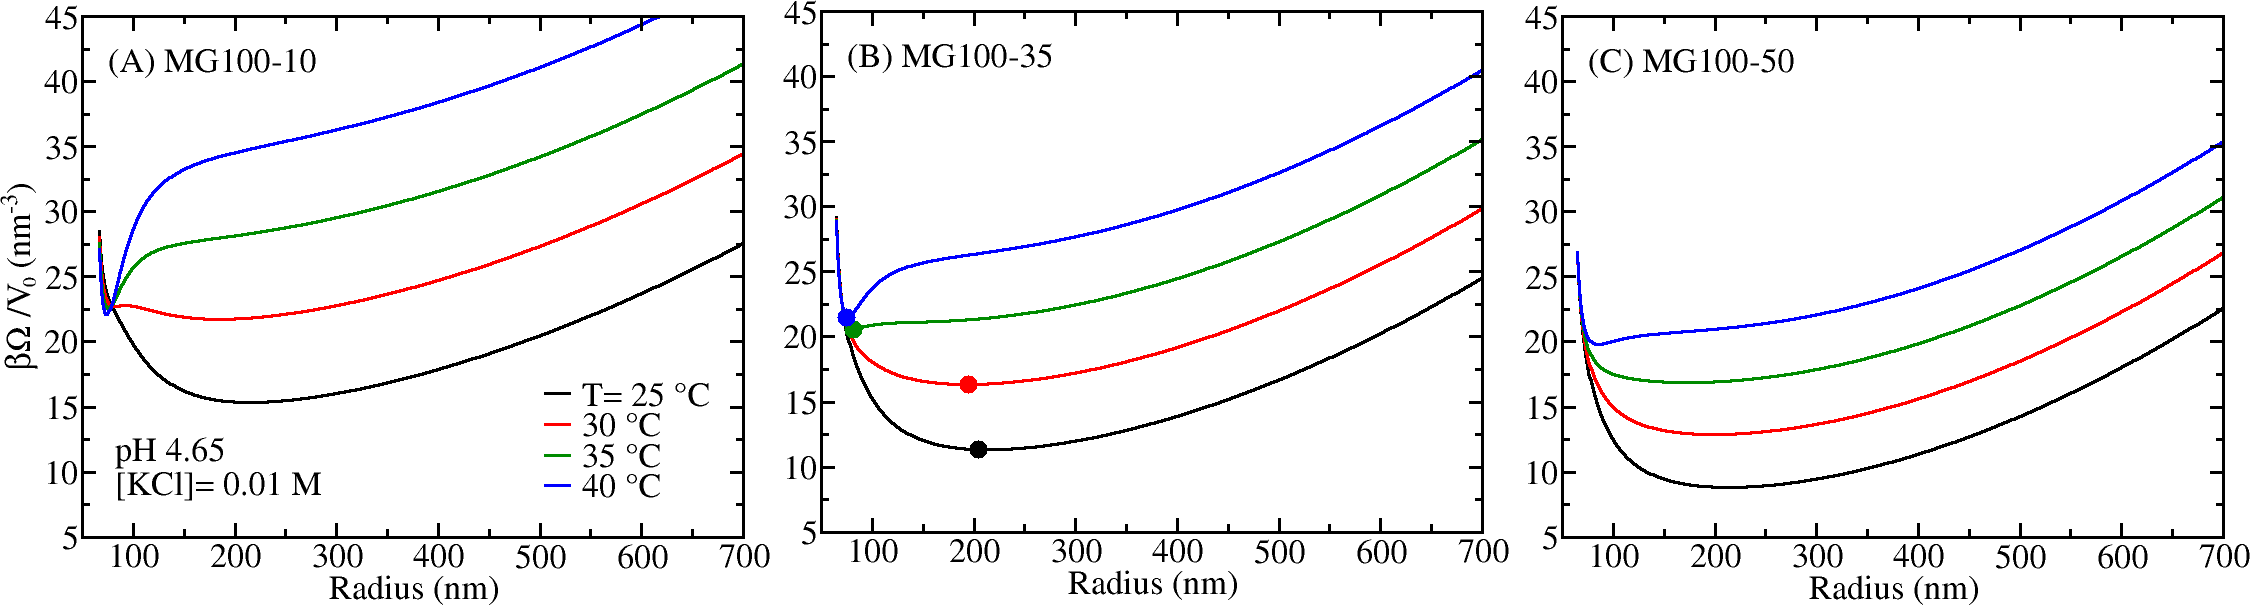
\includegraphics[width=1.\linewidth]{Figures/graph-gel/graph-min.png}
\caption{Potencial termodin\'amico en funci\'on del radio del microgel a diferentes temperaturas, $pH~4.65$ y $cs=10^{-2}M$.
	Cada panel corresponde a un microgel MG100 diferente (longitud de cadena, $n_{ch}=100$) con $10\%$ (A), $35\%$ (B) y $50\%$ (C) MAA.
	Las curvas presentan el potencial termodin\'amico en exceso de la contribuci\'on de la soluci\'on, $\Omega=\Omega_{MG}-\Omega_s$, en algunas unidades convenientes, donde $V_0=\frac{4}{3}\pi R_0^3$ es el volumen de la part\'icula polim\'erica seca.
	En el panel B, los puntos  marcan el radio \'optimo para cada temperatura, que es el m\'inimo local/global de la curva correspondiente (ver tabla \ref{table:optimal-R}).}
\label{fig:graph-min}
\end{figure*}

En este punto, es posible determinar completamente la energí\'ia libre de la fase de microgel para cualquier $R$ dado.
Las variables independientes de un c\'alculo son la temperatura, el pH y la concentraci\'on de sal de la soluci\'on en contacto con la fase microgel.
El n\'umero de segmentos en la red de pol\'imero $N_{seg}$, la longitud de la cadena $n_{ch}$ y la fracci\'on de segmentos MAA, $x_{MAA}$, caracterizan completamente a nuestro microgel.


Consideramos microgeles con $N_{seg}=10^7$ segmentos y $n_{ch}=50$, $100$ y $200$, que tienen $x_{MAA}=0,1$, $0,35$ o $0,5$.
El objetivo es evaluar el efecto de aumentar o reducir la cantidad de mon\'omero \'acido con respecto a los microgeles de poli(NIPAm-\emph{co}-MAA) que tienen $35\%$ MAA. % que normalmente se sintetizan en nuestro laboratorio \addcite[Giussi2015 ,Giussi2020].
Estos microgeles est\'an etiquetados como MG$n_{ch}$-$p_{MAA}$, donde $p_{MAA}$ es el porcentaje de MAA.
Por ejemplo, MG100-10 corresponde a un  microgel con $n_{ch}=100$ y $x_{MAA}=0,1$.


Para determinar el tama\~no del microgel para un conjunto dado de condiciones, recurrimos a una minimizaci\'on gr\'afica del mismo.
Para cada conjunto de condiciones (pH, sal y $T$), construimos $\Omega(R)=\Omega_{MG}(R)-\Omega_{s}(R)$, y encontramos $R_{opt }$, siedo este el radio \'optimo, tal que la curva tenga un m\'inimo local (y global).
Como ejemplo, este procedimiento se ilustra en la figura \ref{fig:graph-min} para microgeles MG100.
Los resultados obtenidos de la minimizaci\'on de las curvas figura \ref{fig:graph-min} se resumen en la tabla \ref{table:optimal-R}.

\begin{table}[!htb]
\centering
\small
  \begin{tabular}{|lccccc|}
   \hline %\multirow{2}{*}{MG100} & 
    %  \multicolumn{4}{c}{Opt. Radius (nm)(MG100)} \\
    	&&   Opt. Radius (nm)(MG100 & && \\
    	\hline
      & {25 $^\circ C$} & {30 $^\circ C$} & {35 $^\circ C$} & {40 $^\circ C$} & {dry, $R_0$} \\
      \hline
    10\% MAA & 215 &  184 &  75  &  74 & 65\\
    35\% MAA &  213 &  193 &  84 & 76 & 64\\
    50\% MAA &  213 & 199 &  172 & 85 & 63\\
    \hline
  \end{tabular}
 \caption{Minimizaci\'on de las curvas de la  figura \ref{fig:graph-min}.
 	Esta tabla resume los radios \'optimos de tres microgeles MG100 a diferentes temperaturas, $pH\,4.65$ y $[KCl]=10^{-2}M$.}
\label{table:optimal-R} 
\end{table}


\subsection{Absorci\'on}
%%%%%%%%%%%%%%%%%%%%%%%%%%%%%%%%%%%%%%%%%%%%%%%%%%%%%%%%%%%%%%%%%%%%%

Nuestro objetivos es poder utilizar estos microgeles como dispositivos inteligentes, entre los que se destaca su uso como trasnportadores de mecidamentos. Para ello es necesario analizar su factibiliad de su la absorci\'on de drogas terapeuticas. En el presente cap\'itulo realizamos el an\'alisis usando como droga modelo a la Doxorubicina y un derivado de ella Daunorubicina. Ambas drogas muy fuertemente empleadas en tratamientos anticancerigenos. 

Para describir la absorci\'on de un analito a la fase de microgel,
al potencial termodin\'amico de la ec. \ref{eq:gel:free-energy} se le adicionan los siguientes t\'erminos:
%
%
%
\begin{align}
\begin{aligned}
\beta&\frac{\Omega_{MG}(R)}{V}= \cdots\\&+ \rho_a\left(\ln\left(\rho_a v_w\right) -1 + \beta\mu^0_a\right) \\
& + \rho_a \sum_\tau n_\tau  \left[g_\tau(\ln g_\tau+ \beta\mu^0_{\tau,p})\right.\\
&\qquad\left.+(1-g_\tau)(\ln (1-g_\tau)+\beta\mu^0_{\tau, d})\right] \\
& +  \left( \rho_a \sum_\tau n_\tau f_\tau q_\tau\right)\beta\psi_{MG}\\
& -\rho_a\beta\mu_a
 -\beta\mu_{H^+} \rho_a \sum_\tau n_\tau g_\tau
\end{aligned}
\label{eq:gel:ads}
\end{align}
%
\noindent en donde primera l\'inea (lado derecho) representa los grados de libertad de traslaci\'on,
donde $\rho_a$ es la densidad num\'erica del analito y $\mu_a^0$ su potencial qu\'imico est\'andar.
Las siguientes dos l\'ineas describen el equilibrio \'acido-base de las unidades titulables del analito;
el sub\'indice $\tau$ recorre dichas unidades moleculares que tienen un grado de protonaci\'on $g_\tau$ y un volumen $v_\tau$.
El analito tiene $n_\tau$ de estos segmentos;
$\mu^0_{\tau, p}$ y $\mu^0_{\tau,d}$ son el potencial qu\'imico est\'andar de las especies protonadas y desprotonadas, respectivamente, que se relacionan con la constante de disociaci\'on \'acida:
%
\begin{align}
K^0_{a,\tau}= e^{\beta\mu^0_{\tau, p}-\beta\mu^0_{\tau,d}-\beta\mu^0_{H^+}}
\end{align}
%

La siguiente l\'inea en la ec. \ref{eq:gel:ads} describe la contribuci\'on del analito a la energ\'ia electrost\'atica, donde $f_\tau$ es el grado de carga de las unidades $\tau$, que es igual a $g_\tau$ si $\tau$ es un grupo b\'asico, o $(1-g_\tau)$ si la unidad es \'acida; $q_\tau$ es la carga de las especies ionizadas.
Los dos \'ultimos t\'erminos dan cuenta del equilibrio qu\'imico entre el microgel y la fase de soluci\'on, donde $\mu_a$ es el potencial qu\'imico del analito.

Adem\'as, la ec. \ref{eq:gel:packing} debe incorporar la fracci\'on total de volumen ocupada por el analito: $\rho_a \sum_\lambda n_\lambda v_\lambda$, donde $\lambda$ recorre todos los tipos de segmentos que forman la mol\'ecula, incluyendo unidades titulables $\{\tau\}\in\{\lambda\}$.
La presencia del analito en la fase de soluci\'on tambi\'en representa contribuciones adicionales al potencial termodin\'amico $\Omega_s$ de ec. \ref{eq:gel:bulk}, que contienen los mismos componentes que ec. \ref{eq:gel:ads}.

De estas \'ultimas dos ecuaciones se reescriben como:

Para la fase gel:
\begin{align}
	\begin{aligned}
		\beta&\frac{\Omega_{MG}(R)}{V}=\\
		& ~ \sum_{\gamma} \rho_\gamma\left(\ln\left(\rho_\gamma v_w\right) -1 + \beta\mu^0_\gamma\right) \\
		%%%
		&+ \rho_a\left(\ln\left(\rho_a v_w\right) -1 + \beta\mu^0_a\right) \\
		%%%
		& + \frac{\phi_{MAA}}{v_{MAA}} \left[f(\ln f+ \beta\mu^0_{MAA^-})\right.\\
		&\qquad\left.+(1-f)(\ln (1-f)+\beta\mu^0_{MAAH})\right] \\
		%
		& + \rho_a \sum_\tau n_\tau  \left[g_\tau(\ln g_\tau+ \beta\mu^0_{\tau,p})\right.\\
		&\qquad\left.+(1-g_\tau)(\ln (1-g_\tau)+\beta\mu^0_{\tau,d})\right] \\
		%%
		& + \dfrac{3}{2}\dfrac{N_{seg}}{n_{ch} V}\left[\left(\dfrac{R}{R_0}\right)^2 - \ln\dfrac{R}{R_0} -1\right] \\
		%
		& +  \left(\sum_{\gamma } {\rho_\gamma q_\gamma + f\dfrac{\phi_{MAA}}{v_{MAA}}q_{MAA}} + \rho_a \sum_\tau n_\tau f_\tau q_\tau \right)\beta\psi_{MG}\\
		%
		& +\beta\pi_{MG} \left[ \sum_{\gamma } \rho_\gamma v_\gamma  + \phi_{MAA} + \phi_{NIPAm} + \rho_a \sum_\lambda n_\lambda v_\lambda -1 \right] \\
		%
		& + \chi (T, \phi_{NIPAm})\rho_w \phi_{NIPAm} \\
		%
		& -\sum_{\gamma }{\rho_\gamma\beta\mu_\gamma} -\rho_a\beta\mu_a
		-\beta\mu_{H^+}(1-f)\dfrac{\phi_{MAA}}{v_{MAA}} 
		-\beta\mu_{H^+} \rho_a \sum_\tau n_\tau g_\tau\\
		%
		%
	\end{aligned}
	\label{eq:gel:total}
\end{align}
En las cuales las nuevas restricciones para la fase gel son:

\begin{align}
	1 = \sum_{\gamma } \rho_\gamma v_\gamma  + \phi_{MAA} + \phi_{NIPAm} + \rho_a \sum_\lambda n_\lambda v_\lambda
	\label{eq:gel:packing-g-total}
\end{align}

y 

\begin{align}
	\sum_{\gamma } {\rho_\gamma q_\gamma + f\dfrac{\phi_{MAA}}{v_{MAA}}q_{MAA}} + \rho_a \sum_\tau n_\tau f_\tau q_\tau = 0
\end{align}

Para la fase soluci\'on:

\begin{align}
	\begin{aligned}
		\beta&\frac{\Omega_s}{V}=\\& \sum_{\gamma   } {\rho^s_\gamma\left(\ln(\rho_\gamma^sv_w) -1 + \beta\mu_\gamma^0 - \beta\mu_\gamma\right)} \\
		& + \rho^s_a \left( \ln \rho^s_a v_w -1 +\beta\mu^0_a - \beta\mu_a\right)
	\end{aligned}
	\label{eq:gel:bulk-total}
\end{align}

y sus respectivas restricciones:

\begin{align}
	1 = \sum_{\gamma } \rho_\gamma v_\gamma  + \rho_a \sum_\lambda n_\lambda v_\lambda
\end{align}

y 

\begin{align}
	\sum_\gamma \rho_\gamma q_\gamma + \rho_a \sum_\tau n_\tau f_\tau q_\tau = 0
\end{align}



De la optimizaci\'on de nuestro nuevo gran potencial $\Omega_{MG}$  se obtiene:
%
\begin{equation}
\frac{f_\tau}{1-f_\tau}=\left(\frac{a_{H^+}}{K^0_\tau}\right)^{\mp 1} e^{-\beta \psi_{MG} q_\tau}
\label{eq:f_ads}
\end{equation}
%
\noindent para el grado de carga de las unidades $\tau$, donde el signo $\mp$ diferencia el caso de un grupo \'acido ($-$) de uno b\'asico ($+$).
Para la densidad del analito obtenemos:
%
\begin{align}
    \begin{aligned}
   \rho_a v_w =&\frac{ \exp{\left(\beta \mu_a - \beta \mu^0_a \right)}}{\prod_\tau \left(1-f_\tau\right)^{n_\tau}}\\
&\quad \cdot\exp{\left(-\beta \pi_{MG} \sum_\lambda n_\lambda v_\lambda \right)} 
    \end{aligned}\label{eq:rho_ads}
\end{align}
%

\noindent donde esta \'ultima ecuaci\'on requiere una redefinici\'on de $\mu_a$ y $\mu_a^0$. Similar a las expresiones presentadas en el cap\'itulo de films.
Expresiones similares a la ec. \ref{eq:rho_ads} y ec. \ref{eq:f_ads} se derivan para la fase de soluci\'on; y con ellas la obteci\'on de los potenciales (y sus respectivas actividades) de los analitos y especies libres. 



\begin{figure}[!tb]
\centering
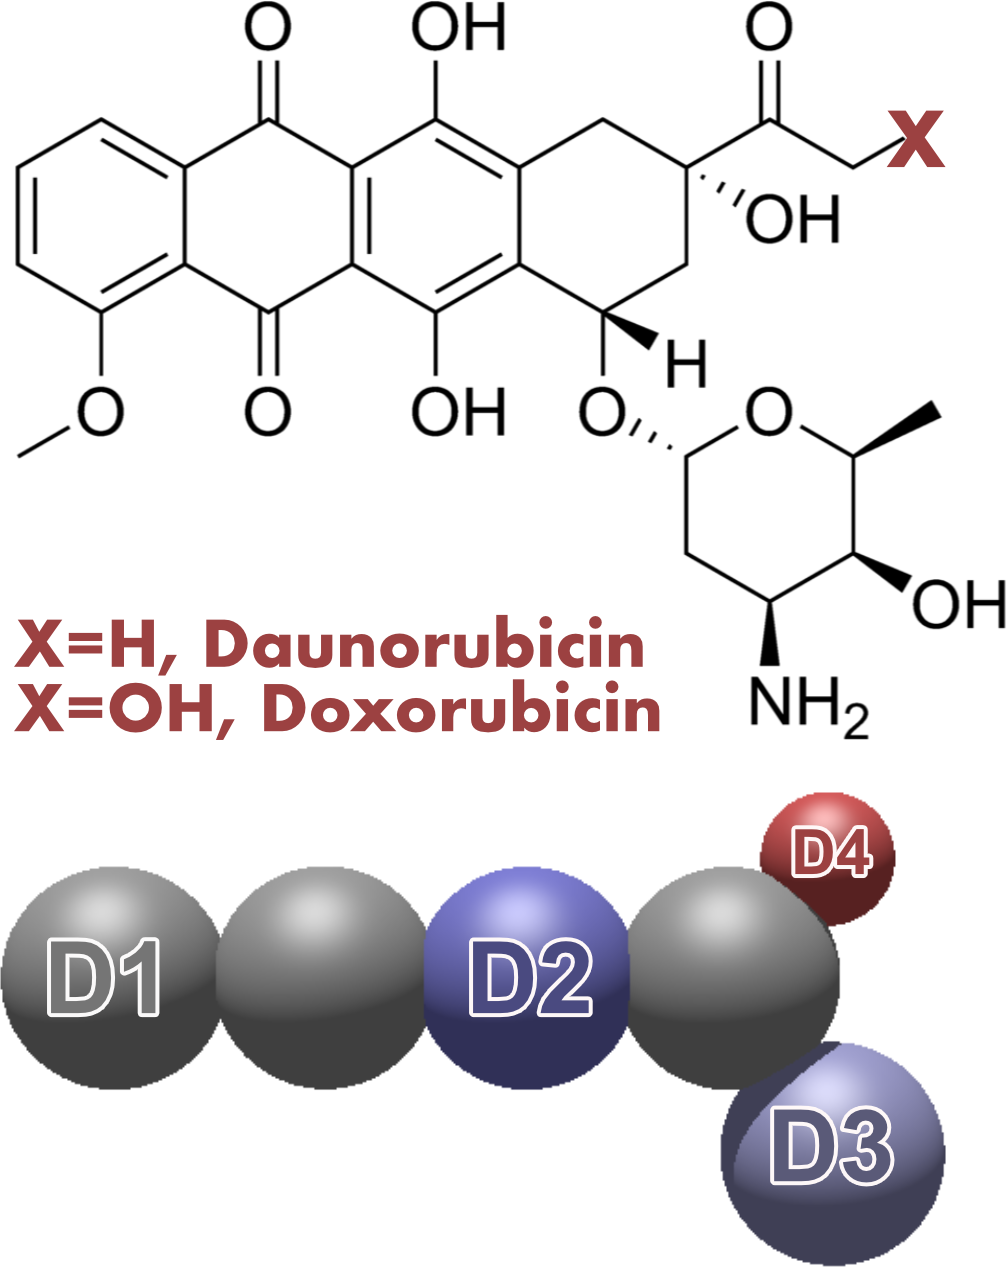
\includegraphics[width=0.35\linewidth]{Figures/graph-gel/dauno-doxo.png}
\caption{Estructura quí\'imica (arriba) y modelo de grano grueso (abajo) aplicado para describir daunorrubicina y doxorrubicina.
	Los segmentos de grano grueso $D1-D4$ se describen en la tabla \ref{table:drugs}.}
\label{fig:dauno-doxo}
\end{figure}


Consideraremos la absorci\'on de los f\'armacos quimioterap\'euticos Daunorrubicina (Dauno) y Doxorrubicina (Doxo) a los microgeles P(NIPAm-MAA) en diferentes condiciones.
El modelo molecular aplicado para describir estos analitos se ilustra en la figura \ref{fig:dauno-doxo} y la parametrizaci\'on se presenta en la tabla \ref{table:drugs} \cite{PerezChavez2020}.

\begin{table}
%\small
%\begin{tabular}{lcS[table-format=-1]S[table-format=0.3]}
\centering
\begin{tabular}{|lccc|}
    \hline
    {CG unit} & {$pKa$} & {$q$ ($e$)} & {$v$ ($\text{nm}^3$)} \\
      \hline
$D1$ & - & 0 & 0.085\\
$D2$ & 7.34 & -1$^\ast$ & 0.085\\
$D3$ & 9.46 & +1$^\ast$ & 0.085\\ 
$D4$ (Doxo) & 8.46 & -1$^\ast$ & 0.035\\
$D4$ (Dauno) & - & 0 & 0.035 \\
    \hline
  \end{tabular}
 \caption{Porpediades moleculares para las distintas unidades de grano grueso usadas para el modelado de las drogas Daunorubicina y Doxorubicina. (ver figura \ref{fig:dauno-doxo}).
\footnotesize ($^\ast$ Para unidades ionizables.)}
\label{table:drugs} 
\end{table}




\section{Resultados y discusi\'on}
%%%%%%%%%%%%%%%%%%%%%%%%%%%%%%%%%%%%%%%%%%%%%%%%%%%%%%%%%%%%%%%%%%%%%



%%%%%%%%%%%%%%%%%%%%%%%%%%%%%%%%%%%%%%%%%%%%%%%%%%%%%%%%%%%%%%%%%%%%%
\subsection{Respuesta al pH y la concentraci\'on de sal}\label{sec:pH_salt}
%%%%%%%%%%%%%%%%%%%%%%%%%%%%%%%%%%%%%%%%%%%%%%%%%%%%%%%%%%%%%%%%%%%%%


\begin{figure}[!ht]
\centering
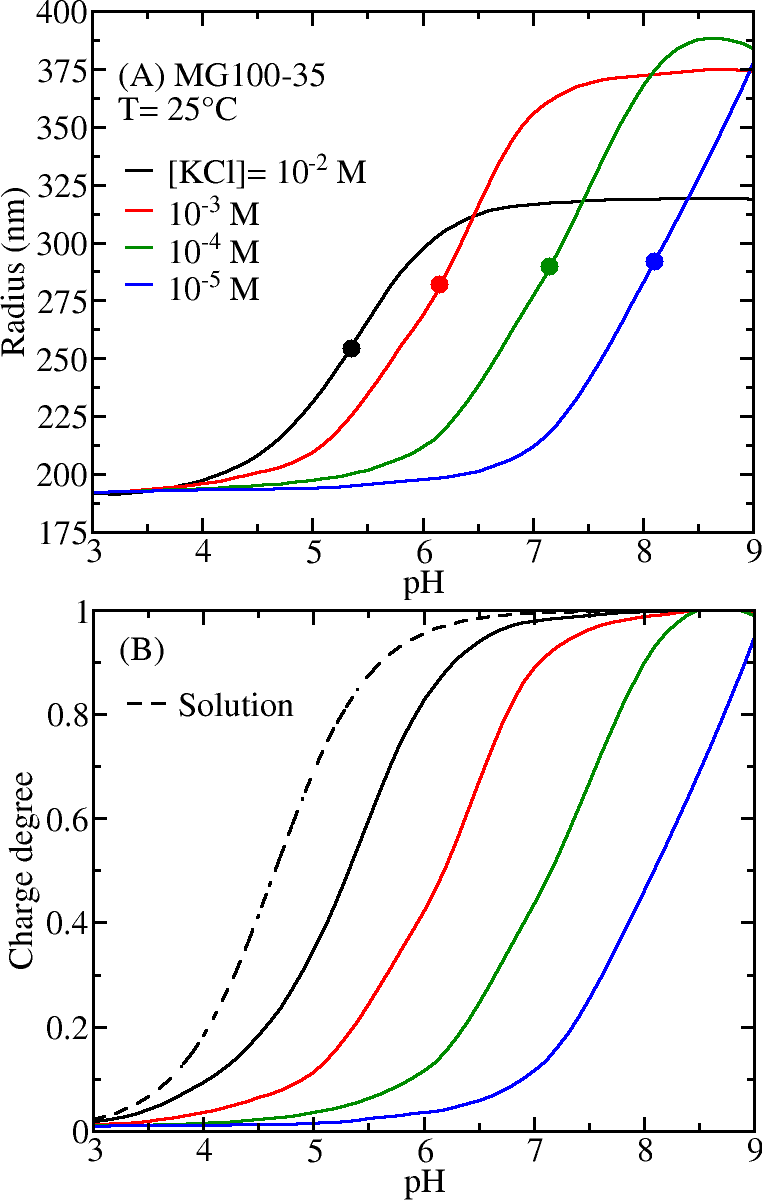
\includegraphics[width=0.5\linewidth]{Figures/graph-gel/R-pH.png}
\caption{Gr\'afico de tama\~no de microgel (A) y grado de carga (B) en funci\'on del pH para soluciones que tienen diferentes concentraciones de sal y $T=25 ^\circ C$.
	Las cadenas de pol\'imero en el microgel MG100-35 son $n_{ch}=100$-long. y tienen $35\% $ MAA.
	La curva de  punteada en el panel B es la disociaci\'on ideal del \'acido metacr\'ilico ($pKa=4.65$).
	Los c\'irculos de color en las curvas del panel A marcan el pKa aparente del microgel.}
\label{fig:R-pH}
\end{figure}

En esta secci\'on, describiremos el comportamiento de los microgeles en respuesta a cambios en la composici\'on de la soluci\'on.
Nos concentramos en temperaturas por debajo de la LCST del PNIPAm;
el efecto de la temperatura se evaluar\'a en \ref{sec:temperature}.


La Figura \ref{fig:R-pH}A muestra el tama\~no del microgel (radio, $R$) en funci\'on del pH para diferentes concentraciones de sal.
Los microgeles de  P(NIPAm-MAA) se hinchan al aumentar el pH.
A medida que aumenta el pH, un n\'umero creciente de unidades MAA se desprotonan y en consecuencia se cargan.
Figura \ref{fig:R-pH}B muestra c\'omo la fracci\'on de MAA cargados ($f$: grado de carga; ver ec. \ref{eq:fcharge}) depende del pH de la soluci\'on.
La hinchaz\'on del microgel observada en el panel A a medida que aumenta el pH es la respuesta a las crecientes repulsiones dentro de la red que resultan del aumento de la carga el\'ectrica en el pol\'imero que se ve en el panel B.


El inicio de la transici\'on de hinchamiento se desplaza a valores de pH m\'as altos cuando se reduce la concentraci\'on de sal (ver fig. \ref{fig:R-pH}A).
Las curvas de disociaci\'on de protones del panel B presentan el mismo desplazamiento a pHs m\'as altos, con respecto al comportamiento ideal de un mon\'omero MAA aislado en soluci\'on diluida.
El pKa aparente de un microgel es el pH al que se desprotonan la mitad de los segmentos MAA;
cuantifica el comportamiento de carga del microgel, fig. \ref{fig:R-pH}B, pero tambi\'en la transici\'on de expansi\'on como vemos en el panel A (ver circulos en $pH=pKa$).
Los pKa aparentes de la fig. \ref{fig:R-pH}B se muestran en la tabla \ref{table:pKa_app}.

\begin{table}[!htb]
\small
  \begin{tabular}{|cc|}
    \hline
      [NaCl] (M)&  pKa app. ($25 ^\circ C$)  \\
      \hline
    $10^{-5}$ & 8.10  \\
    $10^{-4}$ & 7.15 \\
    $10^{-3}$ & 6.15 \\
    $10^{-2}$ & 5.35 \\
    %\azul $10^{-1}$ & \azul 4.80 \\
    ideal (pKa) &  $4.65$  \\
    \hline
  \end{tabular}
 \caption{ pka's aparente de la fig. \ref{fig:R-pH} para un gel MG100-35 a $25 ^\circ C$.}
\label{table:pKa_app} 
\end{table}


Una concentraci\'on relativamente alta de iones de sal dentro del microgel da como resultado el apntallamiento de las repulsiones electrost\'aticas entre los segmentos MAA cargados; estas interacciones repulsivas se vuelven de corto alcance.
Cuando el pH de la soluci\'on aumenta, la disociación de MAA sucede sin un alto costo energ\'etico originado por las repulsiones electrost\'aticas.
En estas condiciones, la desprotonaci\'on de MAA, inducida por la energ\'ia qu\'imica libre (equilibrio \'acido-base), se aproxima al comportamiento ideal o de soluci\'on diluida (compare los casos de alta concenraci\'on salina  con la curva de l\'inea punteada en la fig. \ref{fig:R-pH}B).



Por el contrario, el efecto de apantallamiento se debilita y las repulsiones electrost\'aticas dentro de la red son de mayor alcance para soluciones con baja concentraci\'on de sal.
Incluso si hay pocas cargas y distantes en la red, interactuar\'an entre s\'i.
Para reducir la contribuci\'on energ\'etica de tales repulsiones electrost\'aticas hay un disminuci\'on significatica de que  las unidades MAA se carguen en condiciones de baja salinidad;
en consecuencia el pKa aparente aumenta.
El precio a pagar es aumentar la energ\'ia química libre, cuya contribuci\'on se minimiza cuando el grado de protonaci\'on es ideal.



\begin{figure*}[!htb]
	\centering
	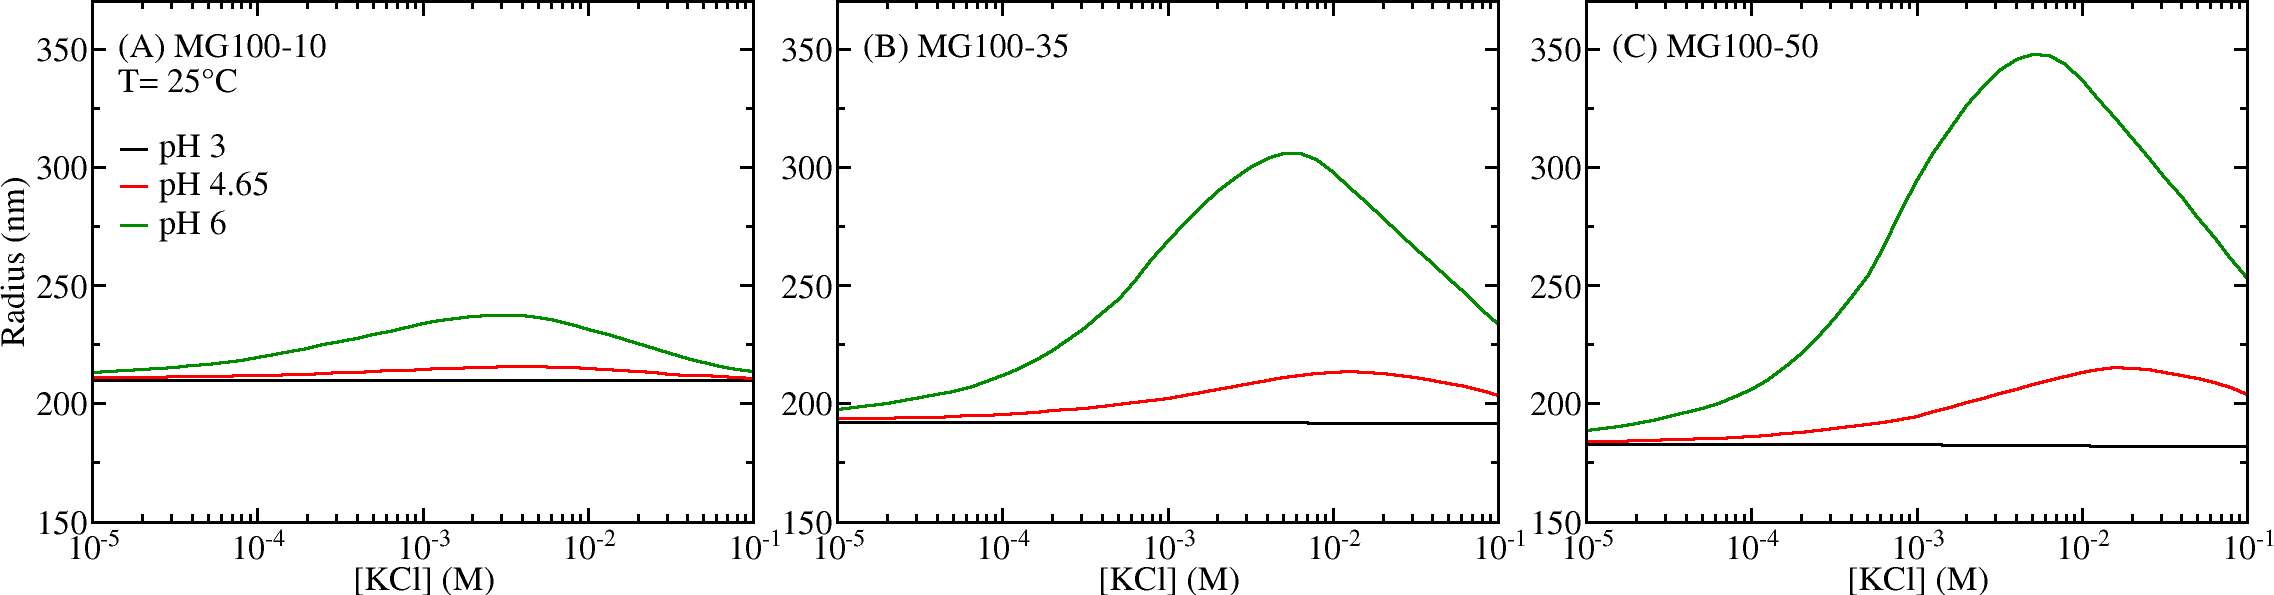
\includegraphics[width=1\linewidth]{Figures/graph-gel/R-cs.png}
	\caption{Gr\'afico del tama\~no del microgel en funci\'on de las concentraciones de sal para diferentes soluciones de pH y $T=25 ^\circ C$.
		Los paneles corresponden a microgeles MG-100 (longitud de cadena, $n_{ch}=100$) que tienen fracciones MAA: $10\%$ (A), $35\%$ (B) y $50\%$ (C).}
	\label{fig:R-cs}
\end{figure*}

La figura \ref{fig:R-cs} ilustra c\'omo el tama\~no de los microgeles de P(NIPAm-MAA) depende de la concentraci\'on de sal para diferentes valores de pH.
A una salinidad relativamente alta, estos microgeles se hinchan con el aumento de la concentraci\'on de sal, lo que es consistente con los resultados de dispersi\'on de luz din\'amica (DLS) de  \cite{Wong2009}para microgeles P(NIPAm-MAA) y concentraciones de KCl en el rango de $0.1-0.5 M$.

Las curvas de la Figura \ref{fig:R-cs} muestran un comportamiento reentrante, en el que el tama\~no primero aumenta y luego disminuye al aumentar la concentración de sal.
Esta respuesta no monot\'onica es m\'as asentuada cuando la carga del pol\'imero aumenta debido a un mayor contenido de pH o MAA (compare diferentes paneles de firgura \ref{fig:R-cs}).



Se han informado transiciones de hinchamiento-deshinchamiento con concentraciones de sal variables en una variedad de sistemas polim\'ericos reguladores de carga.
El grosor de las capas de poli\'acidos d\'ebiles anclados es una funci\'on no monot\'onica de la concentraci\'on de sal de la soluci\'on seg\'un lo predicho por la teor\'ia del campo medio autoconsistente  \cite{Israels1994,Lyatskaya1995,Zhulina1995,Gong2007}, que ha sido confirmada por resultados experimentales \cite{Wu2007}.
De manera similar, los resultados te\'oricos predicen que el tama\~no de los polielectrolitos d\'ebiles ramificados en estrella muestra un m\'aximo en funci\'on de la concentraci\'on de sal en la soluci\'on  \cite{Borisov1998,KleinWolterink2002};
Tambi\'en se ha predicho que el espesor de las pel\'iculas de poliácidos d\'ebiles entrecruzados mostrar\'a este comportamiento de hinchamiento reentrante \cite{Longo2014JCP}.

Se ha predicho una transici\'on deshinchaz\'on a hinchaz\'on impulsada por la sal para los nanogeles de polielectrolitos fuertes \cite{jha2012understanding};
este comportamiento, en el caso de los polielectrolitos ``quencheados'', se atribuy\'o a los efectos de volumen excluidos de los iones absorbidos a altas concentraciones de sal.
M\'as relevante para nuestro estudio, se predijo te\'oricamente una transici\'on de hinchaz\'on a colapso reentrante para microgeles sensibles al pH y al calor \cite{polotsky2013collapse}.
 \citet{polotsky2013collapse} explica que el aumento de la concentraci\'on de sal primero promueve la disociaci\'on de carga de los grupos \'acidos d\'ebiles hasta que se alcanza la saturaci\'on cuando el grado de disociaci\'on alcanza el valor ideal.
M\'as all\'a de este punto, el aumento de la concentraci\'on de sal de la soluci\'on solo mejora el apantallamiento de las repulsiones electrost\'aticas y, por lo tanto, el microgel se deshincha.
Experimentalmente,  \citet{CaprilesGonzalez2008} inform\'o el hinchamiento no monot\'onico de los microgeles de poli(NIPAm-\emph{co}-AA) (P(NIPAm-AA)) en funci\'on de la concentraci\'on de NaCl usando DLS.

\begin{figure}[!tb]
	\centering
	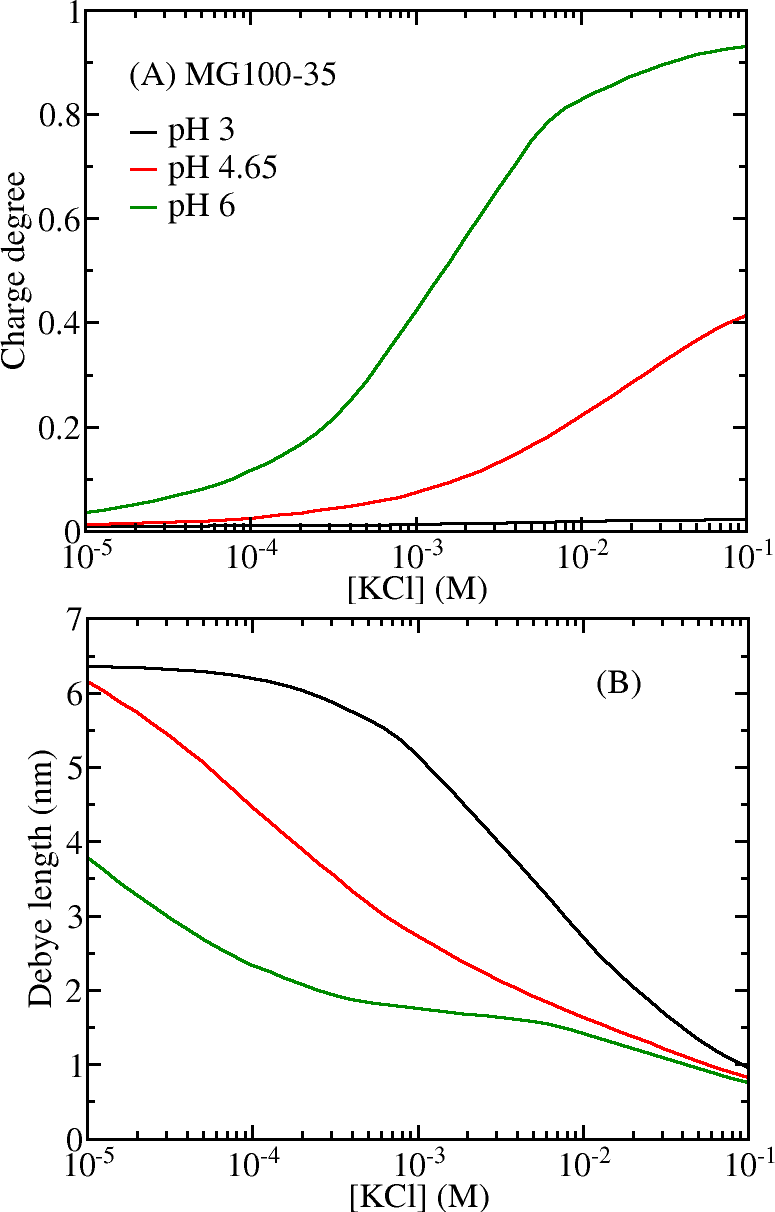
\includegraphics[width=0.5\linewidth]{Figures/graph-gel/f-cs.png}
	\caption{Curvas del grado de carga MAA (A) y la longitud de Debye (B) dentro de los microgeles MG100-35 en funci\'on de la concentraci\'on de sal para diferentes valores de pH.
		Estos resultados corresponden a las condiciones de figura \ref{fig:R-cs}B.}
	\label{fig:f-cs}
\end{figure}



El aumento de la concentraci\'on de sal de la soluci\'on tiene dos efectos opuestos sobre las propiedades del microgel.
Por un lado, aumenta el apantallamiento de interacciones de carga a medida que se cargan los iones dentro del gel; las repulsiones electrost\'aticas entre los mon\'omeros MAA cargados est\'an cada vez m\'as protegidas.
El alcance efectivo de estas repulsiones se acorta favoreciendo el deshinchamiento.
Por otro lado, este apantallamiento permite una mayor desprotonaci\'on de los mon\'omeros MAA, promovida por el equilibrio \'acido-base.
La disociació\'on de carga favorece el hinchamiento para reducir las repulsiones electrostá\'aticas.


La figura \ref{fig:f-cs} ilustra este doble efecto de aumentar la concentraci\'on de sal en la soluci\'on, lo que conduce al comportamiento de hinchamiento-deshinchamiento.
El panel A muestra que la carga del microgel aumenta monó\'otonamente con concentraci\'on de sal.
En el panel B, usamos la longitud de Debye para cuantificar la extensió\'on de las interacciones electrostá\'aticas % (consulte \cref*{si:eq:debye_length} en \supp).
El alcance efectivo de estas interacciones se acorta dentro del microgel a medida que aumenta la concentració\'on de sal.
Puede observarse en la figura \ref{fig:f-cs} que cuando $pH~3$ la carga dentro de la red de polímero es insignificante, lo que resulta en un hinchamiento apreciable en la figura \ref{fig:R-cs}B.



Esta teoria requiere que el interior del microgel sea de carga neutra.
\citet{Claudio2009}demostr\'o que esta es una aproximación razonable cuando el microgel es m\'as grande que $R=125\,\text{nm}$ y tiene un 50\% de mon\'omeros cargados.
Los microgeles P(NIPAm-MAA) de este trabajo son m\'as grandes que ese tama\~no en la mayor\'ia de las condiciones, particularmente cuando el pH está por encima del pKa aparente y la mayor\'ia de los grupos MAA est\'an desprotonados.
Adem\'as, los iones de sal se absorben dentro del microgel para reforzar dicha restricci\'on, lo que permite que los segmentos MAA se desprotonen y se carguen el\'ectricamente.
Describimos este efecto como el apantallamiento de las repulsiones electrost\'aticas entre los grupos MAA, que es un concepto funcional que permite una interpretaci\'on clara de muchas caracter\'isticas del comportamiento de estos microgeles. %\cite{Longo2011}




\subsection{Respuesta a la Temperatura}\label{sec:temperature}
%%%%%%%%%%%%%%%%%%%%%%%%%%%%%%%%%%%%%%%%%%%%%%%%%%%%%%%%%%%%%%%%%%%%%

\begin{figure*}[!htb]
	\centering
	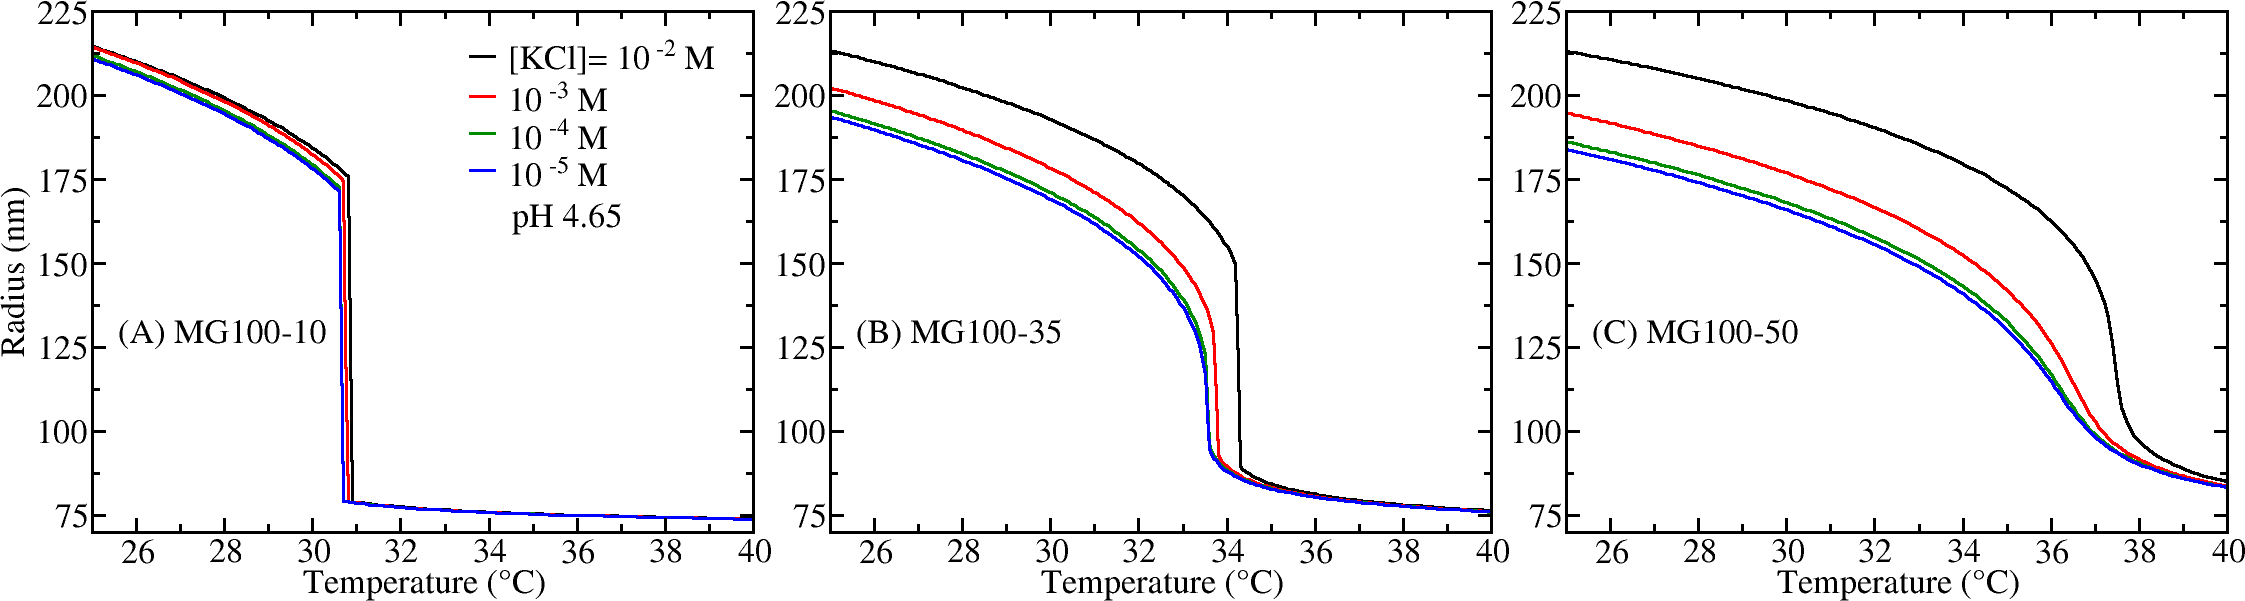
\includegraphics[width=1\linewidth]{Figures/graph-gel/R-T.png}
	\caption{Gr\'afico del tama\~no del microgel en funci\'on de la temperatura para diferentes concentraciones de sal en soluci\'on y $pH~4,65$.
		Los paneles corresponden a microgeles MG-100 (longitud de cadena, $n_{ch}=100$) que tienen diferentes fracciones de MAA: $10\%$ (A), $35\%$ (B) y $50\%$ (C).}
	\label{fig:R-T}
\end{figure*}


En esta secci\'on muestra la respuesta de los microgeles de P(NIPAm-MAA) frente a cambios en la temperatura.
En cada panel de la figura \ref{fig:R-T} se muestra el tama\~no de tres geles MG-100 como funci\'on de la temperatura a distintas concentraciones salinas.
A baja temperatura, estos microgeles muestran un estado relativamente hinchado, mientras que a altas temperaturas se produce un estado colapsado (alta densidad de pol\'imero).


Esto ultimo ocurre dado que el NIPAm adquiere un comportamiento hidrofobico por arriba de su LCST, expulsando el solvente de su interior y colapsando su estructura \cite{sbeih2019structural}.
El tama\~no del gel en este estado es robustamente independiente de la concentraci\'on salina o el pH y posee un radio muy cercano al del microgel seco (ver tabla \ref{table:optimal-R})



Por otro lado, el estado hinchado del gel, es dominado por las repulsiones electrost\'aticas entre los semgemtos de MAA cargados y los contraiones absorvidos, como fue descrito en la secci'on \ref{sec:pH_salt}.
El tama\~no y la carga del microgel son funciones mon\'otonamente decrecientes de
la temperatura.
El estado hinchado se caracteriza por un mayor grado de carga %(ver \cref*{si:fig:f-T} en el \supp).
De hecho, el VPT hinchado a colapsado est\'a acompa\~nado por una transici\'on en el grado de carga de los segmentos MAA.


\begin{figure}[!htb]
	\centering
	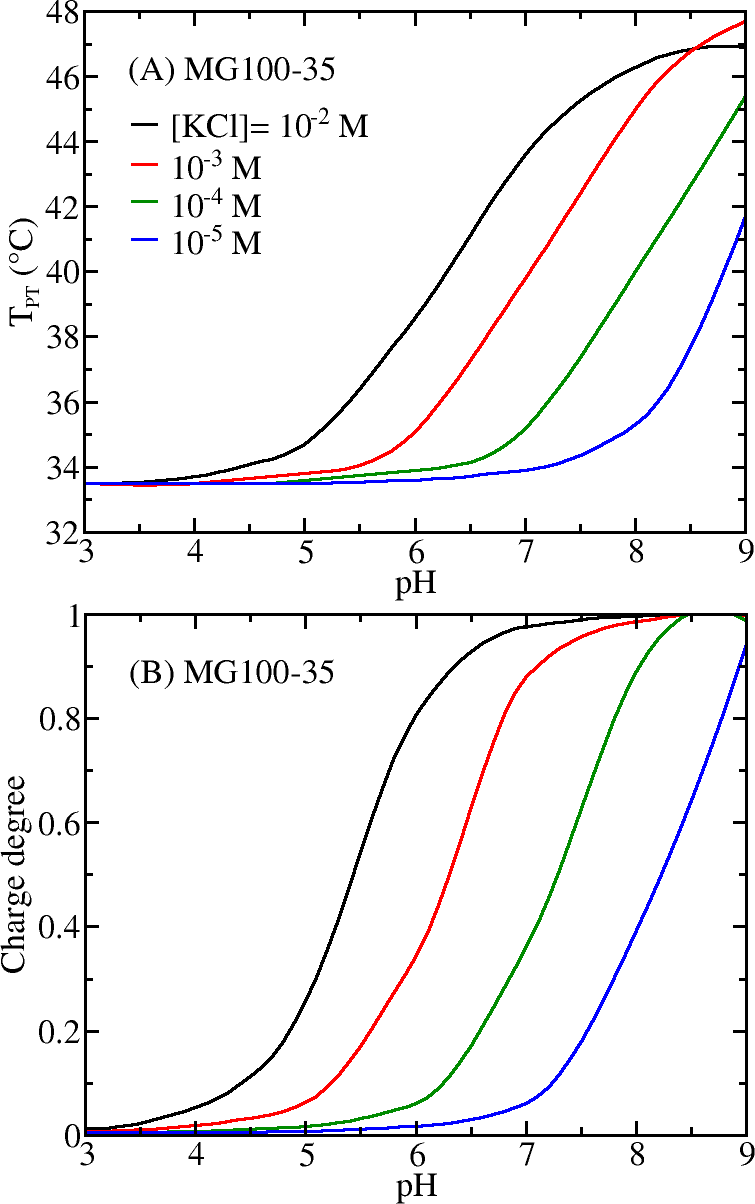
\includegraphics[width=0.5\linewidth]{Figures/graph-gel/Tpt-pH.png}
	\caption{Gr\'aficos que muestran la temperatura de transici\'on de volumen $T_{PT}$ (A) y la fracci\'on de MAA cargado a esta temperatura (B) en funci\'on del pH para diferentes concentraciones de sal.
		Este microgel P(NIPAm-MAA) tiene una longitud de cadena de $n_{ch}=100$ y un MAA de $35\%$.}
	\label{fig:Tpt-pH}
\end{figure}


En la mayor\'ia de las condiciones, pero no en todas, la transici\'on entre estos dos estados del microgel es brusca y ocurre en un rango estrecho alrededor de una temperatura bien definida ($T_{pt}$).
Comparando los diferentes paneles de figura \ref{fig:R-T}, vemos que aumentar el contenido de MAA de los microgeles conduce a una transici\'on m\'as suave alrededor de $T_{pt}$.



La figura \ref{fig:Tpt-pH}A muestra que la $T_{pt}$ aumenta con el pH y la concentraci\'on de sal.
Estos resultados son consistentes con los experimentos DLS que muestran que el VPTT de los microgeles P(NIPAm-MAA) aumenta con el pH \cite{Kleinen2008}, lo que tambi\'en se ha observado para los microgeles P(NIPAm-AA) \cite{CaprilesGonzalez2008}.
Hemos definido $T_{pt}$ como el punto de inflexi\'on de las curvas $R(T)$ de figura \ref{fig:R-T} entre los estados hinchado y colapsado \cite{Kratz2001}.


El panel B de la figura \ref{fig:Tpt-pH} muestra el grado de carga de los segmentos MAA en el $T_{pt}$.
Existe una clara correlaci\'on entre la dependencia de $T_{pt}$ con el pH y la salinidad y el estado de carga del microgel en las condiciones VPT.
La temperatura de transici\'on aumenta con el pH y la concentraci\'on de sal, al igual que la carga de la red de pol\'imeros.

A diferencia de este comportamiento, el VPTT de los microgeles basados en PNIPAm permanentemente cargados disminuye con la concentraci\'on de sal \cite{Lopez2020}.
En este caso, la carga del pol\'imero permanece constante mientras que la incorporaci\'on de iones de sal solo debilita las repulsiones electrost\'aticas entre las cargas.


\begin{figure}[!tb]
	\centering
	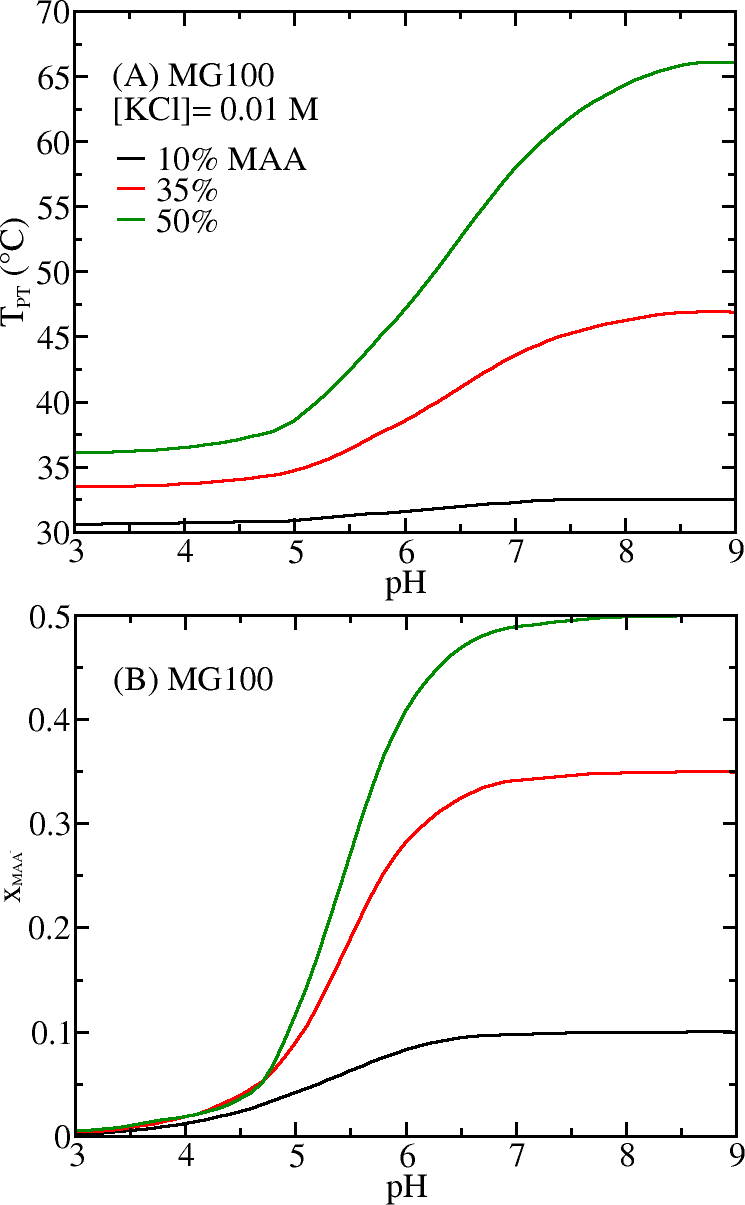
\includegraphics[width=0.5\linewidth]{Figures/graph-gel/Tpt-pH_MAA.png}
	\caption{(A) Gr\'afico de temperatura de transici\'on $T_{PT}$ en funci\'on del pH para microgeles MG-100 (longitud de cadena de pol\'imero, $n_{ch}=100$ segmentos) que tienen diferentes contenidos de MAA; $[KCl]=0.01 M$;
	(B) Fracci\'on de segmentos cargados $x_{MAA^-}=\frac{N_{MAA^-}}{N_{seg}}$ en funci\'on del pH para las mismas condiciones del panel A (\emph{i.e.} , en el $T_{pt}$); $x_{MAA^-}$ es proporcional a la carga total del pol\'imero; $N_{seg}$ es el mismo para todos los microgeles.}
	\label{fig:Tpt_MAA}
\end{figure}


Los resultados de figura \ref{fig:Tpt-pH} muestran que la temperatura de transici\'on est\'a controlada por la cantidad de carga dentro del microgel.
De hecho, aumentar el contenido de MAA tiene el mismo efecto de desplazar el VPTT a valores m\'as altos, como se ve en la figura \ref{fig:Tpt_MAA}A.
Una vez m\'as, este comportamiento resulta de una estructura polim\'erica m\'as cargada.
Para comparar el estado de carga de microgeles con diferentes contenidos de MAA, usamos la fracci\'on total de mon\'omeros cargados:
%
\begin{equation}
x_{MAA^-}=\frac{N_{MAA^-}}{N_{seg}}=f x_{MAA}
\end{equation}
%
\noindent donde $N_{MAA^-}$ es el n\'umero de segmentos MAA desprotonados; todas las dem\'as cantidades se han definido en la sec. \ref{sec:theory};
$x_{MAA^-}$ es proporcional a la carga total de la red de microgel, y
debido a que todos los microgeles tienen el mismo n\'umero total de segmentos, la constante proporcional es la misma para todos los contenidos de MAA considerados.
La figura \ref{fig:Tpt_MAA}B muestra que existe una clara correlaci\'on entre el $T_{pt}$ y la carga total del microgel (dada por $x_{MAA^-}$) al cambiar el pH o el contenido de MAA del pol\'imero.

%%%%%%%%%%%%%%%%%%%%%%%%%%%%%%%%%%%%%%%%%%%%%%%%%%%%%%%%%%%%%%%%%%%%%
\subsection{Efecto del grado de entrecruzamiento}
%%%%%%%%%%%%%%%%%%%%%%%%%%%%%%%%%%%%%%%%%%%%%%%%%%%%%%%%%%%%%%%%%%%%%


\begin{figure*}[!tb]
	\centering
	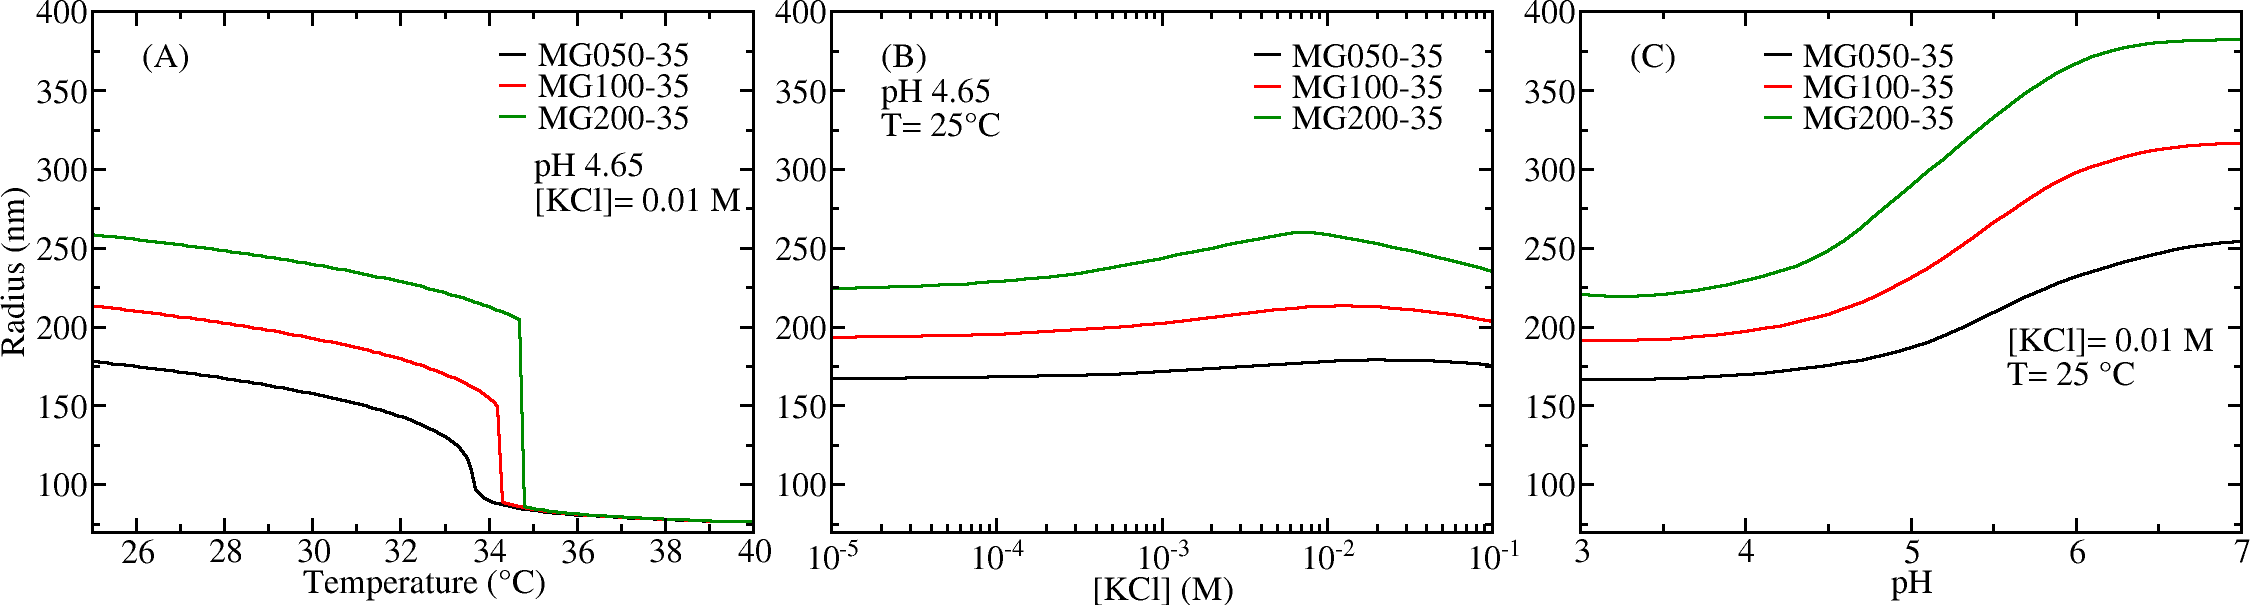
\includegraphics[width=1\linewidth]{Figures/graph-gel/R-all_xlink.png}
	\caption{Gr\'afico del tama\~no del microgel en funci\'on de la temperatura, la concentraci\'on de sal y el pH (paneles A, B y C respectivamente).
		Diferentes curvas corresponden a microgeles con segmentos de $50$ (MG050), $100$ (MG100) y $200$ (MG200) por cadena de pol\'imero, todos con $35\%$ MAA.}
	\label{fig:R_xlink}
\end{figure*}


A continuaci\'on analizamos c\'omo el grado de entrecruzamiento de la red polim\'erica afecta el comportamiento descrito con anterioridad.
Se ha considerado microgeles con segmentos de $50$, $100$ y $200$ por cadena.
Estas part\'iculas tienen el mismo n\'umero total de segmentos.
La figura \ref{fig:R_xlink} muestra la respuesta de los microgeles MAA de $35\%$ a los cambios de temperatura (panel A), concentraci\'on de sal (B) y pH (C).

Los microgeles con menor grado de entrecruzamiento (mayor n\'umero de segmentos por cadena) presentan mayor hinchamiento.
Este comportamiento de los microgeles P(NIPAm-MAA) ha sido confirmado experimentalment  \cite{khan2013preparation}.
Cualitativamente, la respuesta a la concentraci\'on de sal y al pH es similar (paneles B y C de la figura \ref{fig:R_xlink}, respectivamente) para todas las longitudes de cadena consideradas.
Una observaci\'on interesante es que la disminuci\'on del grado de entrecruzamiento conduce a una transici\'on de volumen m\'as brusca cuando aumenta la temperatura (figura \ref{fig:R_xlink}A);
adem\'as la  $T_{pt}$ aumenta.
Nuestros resultados son consistentes con los trabajos de \citet{li1989study} y  \citet{wu1997volume} que informaron un cambio en la transici\'on del volumen de NIPAm de continuo a discontinuo a medida que disminuye la concentraci\'on del entrecruzante en la s\'intesis.


En la figura \ref{fig:R_xlink} tambi\'en vemos que el aumento de la longitud de la cadena (disminuci\'on del grado de entrecruzamiento) desplaza la $T_{pt}$ a temperaturas m\'as altas.
Esto es consistente con los resultados de la espectroscopia UV de  \citet{Lee2008} para microgeles P(NIPAm-AA).
Este comportamiento ocurre para todo el rango de condiciones exploradas en este trabajo %(ver \cref*{si:fig:Tpt-pH_nch} en el \supp, por ejemplo).


La constante de fuerza de la contribuci\'on el\'astica a la energ\'ia libre es inversamente proporcional a la longitud de la cadena $n_{ch}$ (ver eq. \ref{eq:free-energy}).
Al reducir el grado de entrecruzamiento, se hincha el microgel m\'as flexible, lo que permite un mayor grado de carga en la red de pol\'imero.
En consecuencia, se requiere una temperatura m\'as alta para inducir el colapso de la red de pol\'imero.
Hemos demostrado que la $T_{pt}$ est\'a fuertemente correlacionado con el grado de carga.


La presencia de unidades \'acidas acent\'ua la dependencia de  la $T_{pt}$ con la longitud de la cadena porque incorpora el equilibrio de protonaci\'on al juego, pero este comportamiento es intr\'inseco al equilibrio entre las interacciones hidrof\'obicas y la elasticidad de la red.
De hecho, la temperatura de transici\'on de los microgeles de PNIPAm puros tambi\'en aumenta con la longitud de la cadena, aunque el efecto es significativamente m\'as d\'ebil en ausencia de segmentos MAA.


%%%%%%%%%%%%%%%%%%%%%%%%%%%%%%%%%%%%%%%%%%%%%%%%%%%%%%%%%%%%%%%%%%%%%
\subsection{Adsorci\'on de drogas}
%%%%%%%%%%%%%%%%%%%%%%%%%%%%%%%%%%%%%%%%%%%%%%%%%%%%%%%%%%%%%%%%%%%%%

Los microgeles de respuesta m\'ultiple se consideran excelentes candidatos para el desarrollo de veh\'iculos funcionales de administraci\'on de f\'armacos.
Por ejemplo, se sabe que el pH extracelular del tejido tumoral es m\'as bajo que el del tejido sano \cite{Gerweck1996}, lo que hace que los microgeles respondan al pH.
Lo que los hace ideales para la administraci\'on local de medicamentos contra el c\'ancer  \cite{Dadsetan2013}.
%El entorno similar a un tejido dentro de los microgeles puede proporcionar estabilidad a los péptidos o proteínas encapsulados y ayudarlos a retener la actividad tras su liberación\cite{Malmsten2010}.
Adem\'as, para lograr la administraci\'on intestinal del f\'armaco por v\'ia oral,
Peppas \emph{et al.} ha estudiado ampliamente los microgeles sensibles al pH basados en MAA como transportadores inteligentes que pueden operar utilizando los diferentes niveles de acidez a lo largo del tracto digestivo y prevenir la degradaci\'on de f\'armacos en el est\'omago \cite{TorresLugo2002, Carr2010, DuranLobato2014, Sharpe2018}.


En esta secci\'on  evaluamos la capacidad de los microgeles P(NIPAm-MAA) para incorporar dos f\'armacos quimioterap\'euticos.
En particular investigamos las mejores condiciones para la encapsulaci\'on de f\'armacos en condiciones de laboratorio.
Consideramos que la doxorrubicina (Doxo) y la daunorrubicina (Dauno) son dos de las antraciclinas importantes y  amplimanente utilizadas en la quimioterapia para tratar una amplia gama de c\'anceres \cite{Panis2012, Carvalho2009, aubel1984daunorubicin,come1999dual}.
Estas terapias se pueden seguir usando fluorescencia y adsorbancia, lo que las hace atractivas desde el punto de vista de la investigaci\'on \cite{Serpe2005, ThanHtun2009, PerezChavez2020}.
Adem\'as, estos f\'armacos tienen carga positiva en la mayor\'ia de las condiciones, lo que puede facilitar su encapsulaci\'on en microgeles de pol\'imeros ani\'onicos \cite{Li2019}.
\citet{Serpe2005} han estudiado la captaci\'on y liberaci\'on t\'ermicamente activadas de Doxo a partir de pel\'iculas capa por capa de microgeles de P(NIPAm-AA) y poli(clorhidrato de alilamina).
M\'as recientemente, utilizando resonancia magn\'etica nuclear de lapso de tiempo, \citet{MartinezMoro2020} ha descrito la interacci\'on entre Doxo y microgeles P(NIPAm-MAA) en diferentes condiciones.



\begin{figure}[!tb]
	\centering
	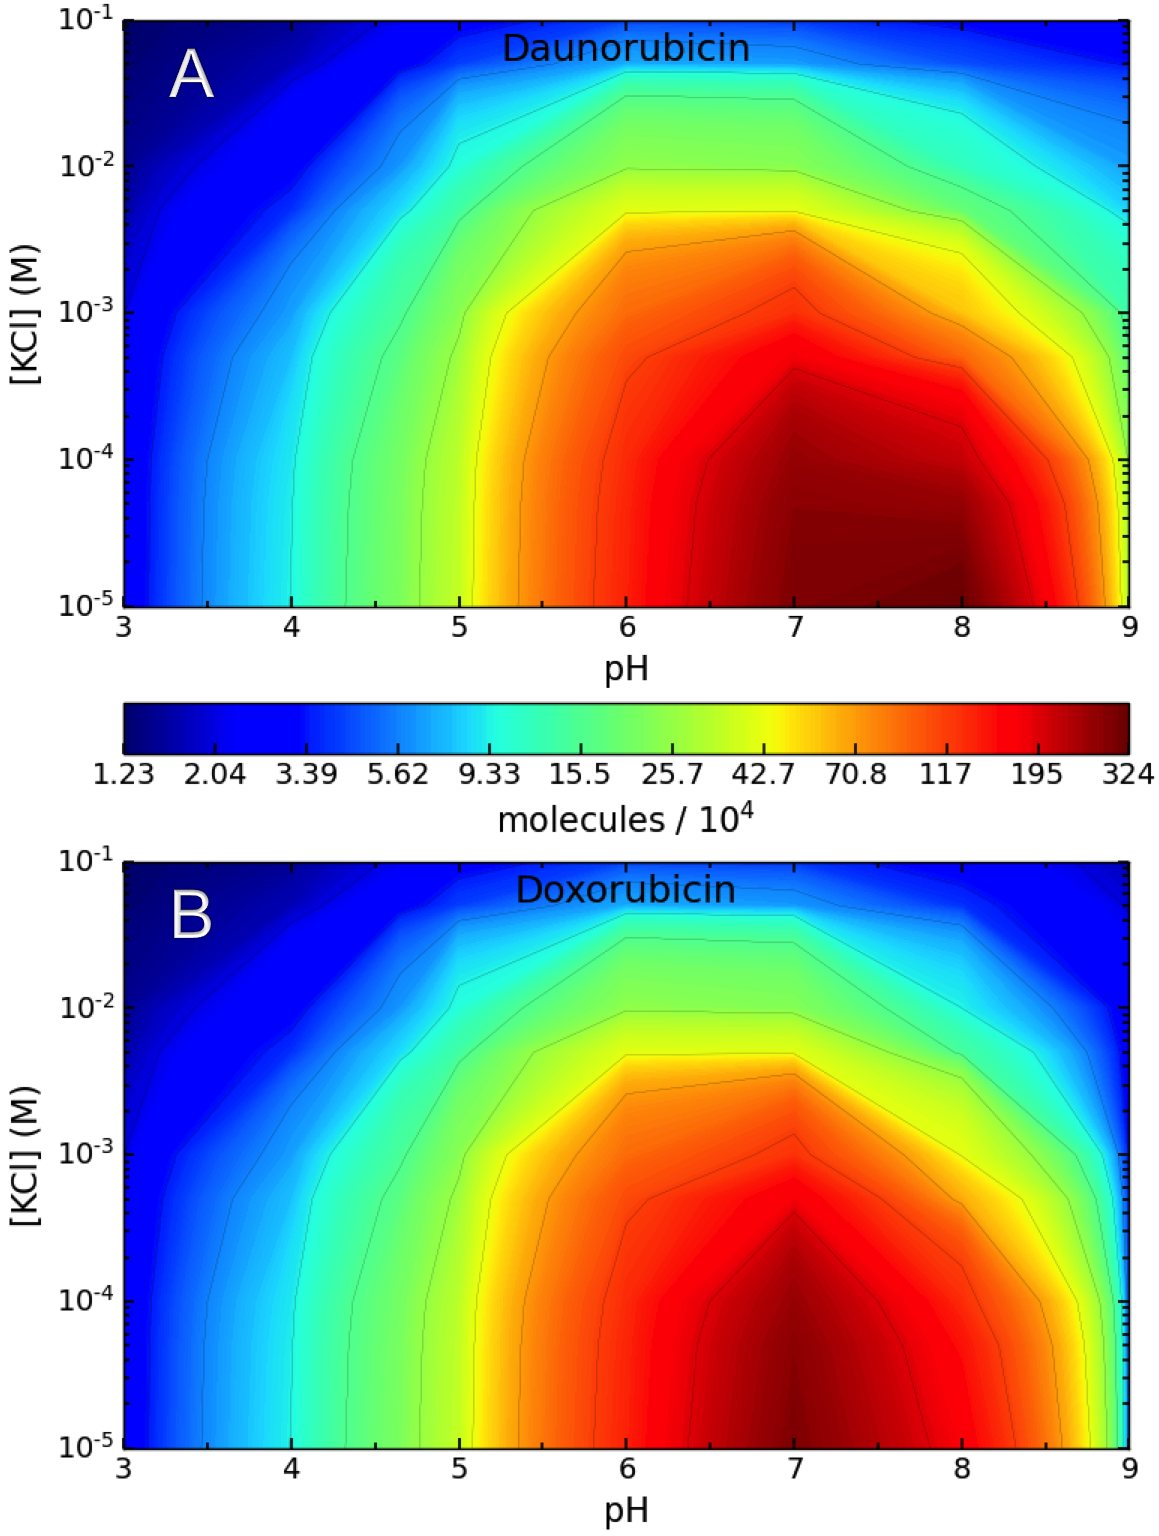
\includegraphics[width=0.55\linewidth]{Figures/graph-gel/drug_ads.png}
	\caption{Mapas en color que muestran el n\'umero de mol\'eculas de daunorrubicina (A) y doxorrubicina (B) absorbidas por microgel en funci\'on del pH de la soluci\'on y la concentraci\'on de sal.
		La concentraci\'on de f\'armaco en soluci\'on es $1mM$ y $T=25 ^\circ C$.
		el microgel P(NIPAm-MAA) tiene $n_{ch}=100$ de longitud de cadena y $35\%$ MAA (MG100-35).}
	\label{fig:drug_ads}
\end{figure}



La figura \ref{fig:drug_ads} muestra el n\'umero de mol\'eculas de Dauno (panel A) y Doxo (panel B) dentro del microgel en funci\'on de la concentraci\'on de sal y el pH de la soluci\'on.
Puede notarse que las mejores condiciones para la encapsulaci\'on de estos f\'armacos terap\'euticos corresponden a baja concentraci\'on de sal y pH $6-8$.
La disminución de la concentraci\'on de sal favorece la absorci\'on.
Tanto Dauno como Doxo tienen una carga neta de $+1$ a un  de pH \'acido y neutro %(consulte \cref*{si:fig:drugs-Q} en el \supp).
Como resultado, su absorci\'on tiene que competir con la de los iones de potasio para neutralizar la carga negativa de la red de pol\'imeros \cite{PerezChavez2020}.
La figura \ref{fig:f-cs} muestra que, en ausencia de un f\'armaco disuelto, la carga del microgel disminuye al disminuir la concentraci\'on de sal, lo que parece entrar en conflicto con la absorci\'on mejorada que se observa en la figura \ref{fig:drug_ads} para estas condiciones .
Sin embargo, tras la absorci\'on del f\'armaco, el grado de carga de los segmentos MAA aumenta significativamente, particularmente en condiciones de bajo contenido de sal %(ver \cref*{si:fig:f-cs_doxo}).
N\'otese tambi\'en que este comportamiento est\'a particularmente asociado con la concentraci\'on de f\'armaco relativamente alta considerada en este trabajo ($1\,$mM).

La fracci\'on de segmentos MAA cargados negativamente en el pol\'imero aumenta con el pH, lo que explica por qu\'e tambi\'en aumenta la absorci\'on de Dauno/Doxo (condiciones \'acidas).
Sin embargo, en condiciones alcalinas, la carga neta positiva de estos f\'armacos disminuye al aumentar el pH, lo que desfavorece la absorci\'on.
Como resultado, la absorci\'on de Dauno/Doxo es una funci\'on no monot\'onica del pH.



En nuestro modelo, los puntos isoel\'ectricos de Dauno y Doxo son $8.4$ y $7.9$, respectivamente% (ver \supp \cref*{si:fig:drugs-Q}).
La figura \ref{fig:drug_ads} muestra que la absorci\'on de ambas mol\'eculas puede ser significativa alrededor y por encima de estos valores de pH.
En otras palabras, existe una absorci\'on considerable de mol\'eculas con carga negativa dentro de la red de polí\'ieros con carga similar.
Aunque, de hecho, estas mol\'eculas est\'an cargadas negativamente en la fase de soluci\'on, la absorci\'on ocurre porque el pH cae dentro del microgel, lo que permite que las drogas regulen su carga el\'ectrica y permanezcan cargadas positivamente dentro del microgel %(\cref*{si:fig:drogas- pH}, \supp).


El punto isoel\'ectrico m\'as bajo de la doxorrubicina se debe a la desprotonaci\'on de su grupo hidroxilo sustituyente (ver $D4$ en figura \ref{fig:dauno-doxo} y tabla \ref{table:drugs}).
Como resultado de esta carga negativa adicional en condiciones alcalinas, el rango de pH de adsorci\'on significativa es ligeramente m\'as amplio para la daunorrubicina.